%%
%% This is file `elsarticle-template-num.tex',
%% generated with the docstrip utility.
%%
%% The original source files were:
%%
%% elsarticle.dtx  (with options: `numtemplate')
%% 
%% Copyright 2007, 2008 Elsevier Ltd.
%% 
%% This file is part of the 'Elsarticle Bundle'.
%% -------------------------------------------
%% 
%% It may be distributed under the conditions of the LaTeX Project Public
%% License, either version 1.2 of this license or (at your option) any
%% later version.  The latest version of this license is in
%%    http://www.latex-project.org/lppl.txt
%% and version 1.2 or later is part of all distributions of LaTeX
%% version 1999/12/01 or later.
%% 
%% The list of all files belonging to the 'Elsarticle Bundle' is
%% given in the file `manifest.txt'.
%% 

%% Template article for Elsevier's document class `elsarticle'
%% with numbered style bibliographic references
%% SP 2008/03/01

%\documentclass[preprint,12pt]{elsarticle}
\documentclass[preprint,10pt]{elsarticle}
%\documentclass[final,3p,times]{elsarticle} 

%% Use the option review to obtain double line spacing
%% \documentclass[authoryear,preprint,review,12pt]{elsarticle}

%% Use the options 1p,twocolumn; 3p; 3p,twocolumn; 5p; or 5p,twocolumn
%% for a journal layout:
%% \documentclass[final,1p,times]{elsarticle}
%% \documentclass[final,1p,times,twocolumn]{elsarticle}
%% \documentclass[final,3p,times]{elsarticle}
%% \documentclass[final,3p,times,twocolumn]{elsarticle}
%% \documentclass[final,5p,times]{elsarticle}
%% \documentclass[final,5p,times,twocolumn]{elsarticle}

%% if you use PostScript figures in your article
%% use the graphics package for simple commands
\usepackage{float}
\usepackage{color}
\usepackage{caption}
\usepackage{subcaption}
%% or use the graphicx package for more complicated commands
\usepackage{graphicx}
%% or use the epsfig package if you prefer to use the old commands
%% \usepackage{epsfig}

%% The amssymb package provides various useful mathematical symbols 
%% The amsthm package provides extended theorem environments
\usepackage{amssymb}
\usepackage{amsmath}
% more math
\usepackage{amsfonts}
\usepackage{amstext}
\usepackage{amsbsy}
\usepackage{mathbbol} 
%% The lineno packages adds line numbers. Start line numbering with
%% \begin{linenumbers}, end it with \end{linenumbers}. Or switch it on
%% for the whole article with \linenumbers.
\usepackage{lineno}

\journal{Journal of Comp. Phys.}
%%%%%%%%%%%%%%%%%%%%%%%%%%%%%%%%%%%%%%%%%%%%%%%%%%%%%%%%%%%%%%%%%%%%
% operators
\renewcommand{\div}{\vec{\nabla}\! \cdot \!}
\newcommand{\grad}{\vec{\nabla}}
% latex shortcuts
\newcommand{\bea}{\begin{eqnarray}}
\newcommand{\eea}{\end{eqnarray}}
\newcommand{\be}{\begin{equation}}
\newcommand{\ee}{\end{equation}}
\newcommand{\bal}{\begin{align}}
\newcommand{\eali}{\end{align}}
\newcommand{\bi}{\begin{itemize}}
\newcommand{\ei}{\end{itemize}}
\newcommand{\ben}{\begin{enumerate}}
\newcommand{\een}{\end{enumerate}}
% DGFEM commands
\newcommand{\jmp}[1]{[\![#1]\!]}                     % jump
\newcommand{\mvl}[1]{\{\!\!\{#1\}\!\!\}}             % mean value
\newcommand{\keff}{\ensuremath{k_{\textit{eff}}}\xspace}
% shortcut for domain notation
\newcommand{\D}{\mathcal{D}}
% vector shortcuts
\newcommand{\vo}{\vec{\Omega}}
\newcommand{\vr}{\vec{r}}
\newcommand{\vn}{\vec{n}}
\newcommand{\vnk}{\vec{\mathbf{n}}}
\newcommand{\vj}{\vec{J}}
\newcommand{\eig}[1]{\| #1 \|_2}

\newcommand{\EI}{\mathcal{E}_h^i}
\newcommand{\ED}{\mathcal{E}_h^{\partial \D^d}}
\newcommand{\EN}{\mathcal{E}_h^{\partial \D^n}}
\newcommand{\ER}{\mathcal{E}_h^{\partial \D^r}}
\newcommand{\reg}{\textit{reg}}

% extra space
\newcommand{\qq}{\quad\quad}
% common reference commands
\newcommand{\eqt}[1]{Eq.~(\ref{#1})}                     % equation
\newcommand{\fig}[1]{Fig.~\ref{#1}}                      % figure
\newcommand{\tbl}[1]{Table~\ref{#1}}                     % table
\newcommand{\sct}[1]{Section~\ref{#1}}                   % section

\newcommand\br{\mathbf{r}}
%\newcommand{\tf}{\varphi}
\newcommand{\tf}{b}

\newcommand{\tcr}[1]{\textcolor{red}{#1}}
\newcommand{\mt}[1]{\marginpar{ {\tiny #1}}}
%%%%%%%%%%%%%%%%%%%%%%%%%%%%%%%%%%%%%%%%%%%%%%%%%%%%%%%%%%%%%%%%%%%%%
%
%   BEGIN DOCUMENT
%
%%%%%%%%%%%%%%%%%%%%%%%%%%%%%%%%%%%%%%%%%%%%%%%%%%%%%%%%%%%%%%%%%%%%%
\begin{document}

 

%%%%%%%%%%%%%%%%%%%%%%%%%%%%%%%%%%%%%%%%%%%%%%%%%%%%%%%%%%%%%%%%%%%%
\begin{frontmatter}

%% Title, authors and addresses

%% use the tnoteref command within \title for footnotes;
%% use the tnotetext command for theassociated footnote;
%% use the fnref command within \author or \address for footnotes;
%% use the fntext command for theassociated footnote;
%% use the corref command within \author for corresponding author footnotes;
%% use the cortext command for theassociated footnote;
%% use the ead command for the email address,
%% and the form \ead[url] for the home page:
%\title{Title\tnoteref{label1}}
%% \tnotetext[label1]{}
%% \author{Name\corref{cor1}\fnref{label2}}
%% \ead{email address}
%% \ead[url]{home page}
%% \fntext[label2]{}
%% \cortext[cor1]{}
%% \address{Address\fnref{label3}}
%% \fntext[label3]{}

%-------------------------
%-------------------------
\title{lo ma}
%-------------------------
%-------------------------

%% use optional labels to link authors explicitly to addresses:
%% \author[label1,label2]{}
%% \address[label1]{}
%% \address[label2]{}

%-------------------------
%-------------------------
\author{Marc O. Delchini\fnref{label1}}
\ead{delchmo@tamu.edu}

\author{Jean C. Ragusa\corref{cor1}\fnref{label1}}
\ead{jean.ragusa@tamu.edu}

\author{Ray A. Berry\fnref{label2}}
\ead{ray.berry@inl.gov}

\address[label1]{Department of Nuclear Engineering, Texas A\&M University, College Station, TX 77843, USA \fnref{label1}}

\address[label2]{Idaho National Laboratory, Idaho Falls, ID 83415, USA \fnref{label2}}

\cortext[cor1]{Corresponding author}
%-------------------------
%-------------------------

%-------------------------
\begin{abstract}

aaa 

\end{abstract}
%-------------------------

%-------------------------
\begin{keyword}
  aaa \sep
	bbb \sep
  ccc
\end{keyword}
%-------------------------

\end{frontmatter}

%%%%%%%%%%%%%%%%%%%%%%%%%%%%%%%%%%%%%%%%%%%%%%%%%%%%%%%%%%%%%%%%%%%%

\linenumbers

%%%%%%%%%%%%%%%%%%%%%%%%%%%%%%%%%%%%%%%%%%%%%%%%%%%%%%%%%%%%%%%%%%%%%%%%%%%%%%%%%%%%%%%%%%%%%%%%%%%%
%%%%%%%%%%%%%%%%%%%%%%%%%%%%%%%%%%%%%%%%%%%%%%%%%%%%%%%%%%%%%%%%%%%%%%%%%%%%%%%%%%%%%%%%%%%%%%%%%%%%
\section{Introduction} \label{sec:intro}
%%%%%%%%%%%%%%%%%%%%%%%%%%%%%%%%%%%%%%%%%%%%%%%%%%%%%%%%%%%%%%%%%%%%%%%%%%%%%%%%%%%%%%%%%%%%%%%%%%%%
%%%%%%%%%%%%%%%%%%%%%%%%%%%%%%%%%%%%%%%%%%%%%%%%%%%%%%%%%%%%%%%%%%%%%%%%%%%%%%%%%%%%%%%%%%%%%%%%%%%%
Over the past years an increasing interest raised for computational methods that can solve both compressible and incompressible flows. In engineering applications, there is often the need to solve for complex flows where a near incompressible regime or low Mach flow coexists with a supersonic flow domain. For example, such flow are encountered in aerodynamic in the study of airships. In the nuclear industry, flows are nearly the incompressible regime but compressible effects cannot be neglected because of the heat source and thus needs to be accurately resolved. \\
Because of the hyperbolic nature of the flow equations, numerical methods are required in order to accurately resolve shocks that can form during transonic and supersonic flows. Numerous numerical methods are available in the literature: flux-limiter, pressure-based viscosity method, Lapidus method, the entropy-viscosity method among others. These numerical methods are usually tested and developed using simple equation of states and for transonic and supersonic flows where the disparity between the acoustic waves and the fluid speed is not large since the Mach number is of order one.  
%%%%%%%%%%%%%%%%%%%%%%%%%%%%%%%%%%%%%%%%%%%%%%%%%%%%%%%%%%%%%%%%%%%%%%%%%%%%%%%%%%%%%%%%%%%%%%%%%%%%
%%%%%%%%%%%%%%%%%%%%%%%%%%%%%%%%%%%%%%%%%%%%%%%%%%%%%%%%%%%%%%%%%%%%%%%%%%%%%%%%%%%%%%%%%%%%%%%%%%%%
\section{The Entropy Viscosity Method} \label{sec:entro_visc}
%%%%%%%%%%%%%%%%%%%%%%%%%%%%%%%%%%%%%%%%%%%%%%%%%%%%%%%%%%%%%%%%%%%%%%%%%%%%%%%%%%%%%%%%%%%%%%%%%%%%
%%%%%%%%%%%%%%%%%%%%%%%%%%%%%%%%%%%%%%%%%%%%%%%%%%%%%%%%%%%%%%%%%%%%%%%%%%%%%%%%%%%%%%%%%%%%%%%%%%%%

%===================================================================================================
\subsection{Background} \label{sec:background}
%===================================================================================================
In this section, the entropy-based viscosity method \cite{jlg1, jlg2, jlg3} is recalled for the multi-D Euler equations (with constant area $A$) \cite{valentin}. As mentioned in \sct{sec:intro} the entropy-based viscosity method consists of adding dissipative terms, with a viscosity coefficient modulated by the entropy production which allows high-order accuracy when the solution is smooth. Thus, two questions arise: (i) how are the viscosity dissipative terms derived and (ii) how to numerically compute the entropy production. Answers to the first question can be found in \cite{jlg} by Guermond et al., that details the proof leading to the derivation of the artificial dissipative terms (\eqt{eq:euler_visc}) consistent with the entropy minimum principle theorem. The viscous regularization obtained is valid for any equation of state as long as the opposite of the physical entropy function is convex.
\begin{equation}
\label{eq:euler_visc}
\left\{ 
\begin{array}{lll}
\partial_t \left( \rho \right) + \div \left( \rho \vec{u} \right) = \div \left( \kappa \grad \rho \right) \\
\partial_t \left( \rho \vec{u} \right) + \div \left( \rho \vec{u} \otimes \vec{u} + P \mathbf{I} \right) = \div \left( \mu \rho \grad^s \vec{u}  + \kappa \vec{u} \otimes \grad \rho \right)  \\
\partial_t \left( \rho E \right) + \div \left[ \vec{u} \left( \rho E + P \right) \right] = \div \left( \kappa \grad \left( \rho e \right) + \frac{1}{2}|| \vec{u} ||^2 \kappa \grad \rho +  \rho \mu \vec{u} \grad \vec{u}  \right) \\
P = P\left( \rho, e \right)
\end{array}
\right.
\end{equation}
where $\kappa$ and $\mu$ are local positive viscosity coefficients. \\
The existence of a specific entropy $s$, function of the density $\rho$ and the internal energy $e$ is assumed. Convexity of $-s$ with respect to $e$ and $1/\rho$ is required, along with the following equality verified by the partial derivatives of $s$ : $P \partial_e s + \rho^2 \partial_{\rho} s = 0$.\\
One crucial step remains a definition for the local viscosity coefficients $\mu$ and $\kappa$. In the current version of the method, $\kappa$ and $\mu$ are set equal, so that the above viscous regularization (\eqt{eq:euler_visc}) is equivalent to the parabolic regularization \cite{Parabolic}. The current definition includes a first-order viscosity coefficient referred to with the subscript $max$, and a high-order viscosity coefficient referred to with the subscript $e$. The first-order viscosity coefficients $\mu_{max}$ and $\kappa_{max}$ are proportional to the local largest eigenvalue $|| \vec{u} || + c $ and equivalent to an upwind-scheme, when used, which is known to be over-dissipative and monotone \cite{Toro}: 
\begin{equation}
\mu_{max}(\vec{r}, t) = \kappa_{max}(\vec{r}, t) = \frac{h}{2} \left( || \vec{u} || + c \right),
\end{equation}
where $h$ is the spatial grid size. \\
The second-order viscosity coefficients $\kappa_e$ and $\mu_e$ are set proportional to the entropy production that is evaluated by computing the local entropy residual $D_e$. It also includes the interfacial jump of the entropy flux $J$ that will allow to detect any discontinuities other than shocks:
\begin{equation}
\label{eq:ent_visc_coeff}
\mu_e(\vec{r},t) = \kappa_e(\vec{r},t) = h^2 \frac{\max\left( | D_e(\vec{r},t) |, J \right)}{|| s - \bar{s} ||_{\infty}} \text{ with } D_e(\vec{r}, t) = \partial_t s + \vec{u} \cdot \grad s
\end{equation}
where $|| \cdot ||_{\infty}$ and $\bar{\cdot}$ denote the infinite norm operator and the average operator over the entire computational domain, respectively. The definition of the jump $J$ is discretization-dependent and examples of definition can be found in \cite{valentin} for DGFEM. The denominator $|| s - \bar{s} ||_{\infty}$ is used for dimensionality purposes and should not be of the same order as $h$, on penalty of loosing the high-order accuracy. Currently, there are no theoretical justification for choosing the denominator. \\
The definition of the viscosity coefficients $\mu$ and $\kappa$ is function of the first- and second-order viscosity coefficients as follows:
\begin{equation}
\mu(\vec{r},t) = \min\left( \mu_e(\vec{r},t), \mu_{max}(\vec{r},t) \right) \text{ and } \kappa(\vec{r},t) = \min\left( \kappa_e(\vec{r},t), \kappa_{max}(\vec{r},t) \right).
\end{equation}
This definition allows the following properties.
In shock regions, the second-order viscosity coefficient experiences a peak because of entropy production, and thus, saturates to the first-order viscosity that is known to be over-dissipative and will smooth out oscillations. Anywhere else, the entropy production being small, the viscosity coefficients $\mu$ and $\kappa$ are of order $h^2$.\\
Using the above definition of the entropy-based viscosity method, high-order accuracy was demonstrated and excellent results were obtained with 1-D Sod shock tubes and various 2-D tests \cite{jlg1, jlg2, valentin}.
%===================================================================================================
\subsection{Issues in the Low-Mach Regime} 
%===================================================================================================
In the Low-Mach Regime, the flow is known to be isentropic resulting in very little entropy production. Since the entropy viscosity method is directly based on the evaluation of the local entropy production, it will be interested to study how the entropy viscosity coefficients $\mu$ and $\kappa$ scale in the low Mach regime. Mathematically, it means that the entropy residual $D_e$ will be very small, so will be the denominator $|| s - \bar{s} ||_{\infty}$, thus making the ratio, used in the definition of the viscosity coefficients \eqt{eq:ent_visc_coeff}, undetermined.  Therefore, the current definition of the viscosity coefficients seems unadapted to subsonic flow and could lead to ill-scaled dissipative terms. A solution would be to recast the entropy residual as a function of other variables in order to have more freedom in the choice of the normalization parameter. The idea is to still define the viscosity coefficient proportional to the entropy residual that is a good indicator of the flow type (subsonic or supersonic).
%===================================================================================================
\subsection{The dissipative-terms for the multi-D Euler equations with variable area} 
%===================================================================================================
One of the focus of this paper is to investigate the application of the entropy viscosity method to the multi-D Euler equations with variable area: first, the dissipative terms are derived following (REF), and, the viscosity coefficients are defined. The full derivation can be found in APPENDIX and only the main steps are given here. The objective here is to assess wether or not the entropy viscosity method will accurately resolve a flow in a $1$-D convergent-divergent nozzle (REFS with mine). In \sct{sec:results}, $1$-D results for liquid water in a nozzle are shown. This test is interested for two reasons: (i) the flow under consideration is subsonic which is the focus of this paper, and, (ii) the flow reaches a steady-state and an exact-solution can be derived for this particular case (REF). Thus, a convergence study will be performed in order to show second-order accuracy. \\
The multi-D Euler equations degenerate to the multi-D Euler equations given in \eqt{eq:euler_visc} when assuming constant area. The main difference lies in the momentum equation that contains a non-conservative terms in the right-hand side. For the purpose of this paper, the variable area is denoted by $A(\vec{r})$ and is only spatial dependent. The multi-D Euler equations with variable area are recalled (REF):
\begin{equation}
\label{eq:euler_variable_A}
\left\{ 
\begin{array}{lll}
\partial_t \left( \rho A \right) + \div \left( \rho \vec{u} A \right) = 0 \\
\partial_t \left( \rho \vec{u} A \right) + \div \left[A\left( \rho \vec{u} \otimes \vec{u} + P \mathbf{I} \right) \right] = P \grad A \\
\partial_t \left( \rho E \right) + \div \left[ \vec{u} \left( \rho E + P \right) \right] = 0
\end{array}
\right.
\end{equation}
This system (\eqt{eq:euler_variable_A}) admits the following entropy equation with the same entropy function as defined previously in \sct{sec:background}:
\begin{equation}
\rho A \left( \partial_t s + \vec{u} \cdot \grad s \right) = 0 \nonumber
\end{equation}
Once again, by adding dissipative terms in each equation of \eqt{eq:euler_variable_A}, the entropy equation is modified and by invoking the entropy minimum principle, adequate definition of the dissipative terms are derived as shown in \eqt{eq:euler_variable_A_bis}:
\begin{equation}
\label{eq:euler_variable_A_bis}
\left\{ 
\begin{array}{lll}
\partial_t \left( \rho A \right) + \div \left( \rho \vec{u} A \right) = \div \left( A \kappa \grad \rho \right) \\
\partial_t \left( \rho \vec{u} A \right) + \div \left[A\left( \rho \vec{u} \otimes \vec{u} + P \mathbf{I} \right) \right] = P \grad A + \div \left[ A \left( \mu \rho \grad^s \vec{u}  + \kappa \vec{u} \otimes \grad \rho \right) \right]\\
\partial_t \left( \rho E \right) + \div \left[ \vec{u} \left( \rho E + P \right) \right] = \div \left[ A \left( \kappa \grad \left( \rho e \right) + \frac{1}{2}|| \vec{u} ||^2 \kappa \grad \rho +  \rho \mu \vec{u} \grad \vec{u}  \right) \right]
\end{array}
\right.
\end{equation}
The dissipative terms are very similar to the ones obtained for the multi-D Euler equations: each dissipative flux is multiplied by the variable area $A$ in order to  ensure conservation of the flux. When assuming a constant area, \eqt{eq:euler_visc} is retrieved.\\
The definition of the viscosity coefficients is explained in \sct{sec:lowMach}. It is expected to have the same definition of the viscosity coefficients between the multi-D Euler equations with variable and constant area. This assumption is justified by the entropy residual for the variable area case: it can be obtained by simply multiplying the entropy residual of \eqt{eq:ent_visc_coeff} by the area $A$. Thus, the variations of the entropy residual should be identical.  
%%%%%%%%%%%%%%%%%%%%%%%%%%%%%%%%%%%%%%%%%%%%%%%%%%%%%%%%%%%%%%%%%%%%%%%%%%%%%%%%%%%%%%%%%%%%%%%%%%%%
%%%%%%%%%%%%%%%%%%%%%%%%%%%%%%%%%%%%%%%%%%%%%%%%%%%%%%%%%%%%%%%%%%%%%%%%%%%%%%%%%%%%%%%%%%%%%%%%%%%%
\section{All-speed Reformulation of the Entropy Viscosity Method} \label{sec:extension}
%%%%%%%%%%%%%%%%%%%%%%%%%%%%%%%%%%%%%%%%%%%%%%%%%%%%%%%%%%%%%%%%%%%%%%%%%%%%%%%%%%%%%%%%%%%%%%%%%%%%
%%%%%%%%%%%%%%%%%%%%%%%%%%%%%%%%%%%%%%%%%%%%%%%%%%%%%%%%%%%%%%%%%%%%%%%%%%%%%%%%%%%%%%%%%%%%%%%%%%%%
In this section, it is shown how the entropy residual $D_e$ can be recast as a function of the pressure, the density and the speed of sound. Then, an low Mach asymptotic study of the multi-D Euler equations is performed in order to derive the correct normalization parameter. 
%===================================================================================================
\subsection{New Entropy Production Residual} 
%===================================================================================================
The first step in defining a viscosity coefficient that behaves well in the low mach limit is to recast the entropy residual in terms of thermodynamic variables:
\begin{equation}
\label{eq:ent_res}
D_e(\vec{r},t) = \partial_t s + \vec{u} \cdot \grad s = \frac{s_e}{P_e} \left( \underbrace{\frac{d P}{dt} - c^2 \frac{d \rho}{dt}}_{\tilde{D}_e(\vec{r},t)} \right),
\end{equation} 
where $\frac{d \cdot}{dt}$ denotes the material or total derivative, and $P_e$ is the partial derivative of pressure with respect to internal energy. The steps that lead to the new formulation of the entropy residual $D_e$ can be found in APPENDIX. \\
The entropy residual $D_e$ and $\tilde{D}_e$ are proportional to each other and therefore will experience the same variation when taking the absolute value. Thus,  locally evaluating $\tilde{D}_e$ instead of $D_e$ should allow us to measure the entropy production point wise. This new expression given in \eqt{eq:ent_res} has multiple advantages:
\begin{itemize}
\item an analytical expression of the entropy function is not longer needed: the entropy residual $\tilde{D}_e$ is evaluated using the local values of the pressure, the density and the speed of sound. Deriving an entropy function for some complex equation of states can be difficult.
\item with the proposed expression of the entropy residual function of pressure and density, additional normalizations suitable for low Mach flows of the entropy residual can be devised. Examples include the pressure itself, or combination of the density, the speed of sound and the norm of the velocity: $\rho c^2$, $\rho c || \vec{u} ||$ and $\rho || \vec{u} ||^2$. 
\end{itemize}
The viscosity coefficients $\mu$ and $\kappa$ are now defined proportional to the new entropy residual $\tilde{D}_e$ on the model of \eqt{eq:ent_visc_coeff} as follows:
\begin{equation}
\mu \left( \vec(r),t \right) = \kappa \left( \vec(r),t \right) = h^2 \frac{\max \left( \tilde{D}_e, J \right)}{n(P)}
\end{equation}
where $n(P)$ is a normalization parameter to determine and all other variables were defined previously. \\
As mentioned earlier, the normalization parameter $n(P)$ must be of the same units as the pressure for the viscosity coefficients to have the unit of a dynamic viscosity $(m^2 / s)$. Multiples options are available to us ($P$, $\rho c^2$, $\rho c || \vec{u} ||$ and $\rho || \vec{u} ||^2$). The choice of the normalization parameter cannot be random if the definition of the viscosity coefficient is wanted to be well-scaled for a wide range of Mach numbers. For example, by choosing $n(P) = \rho || \vec{u} ||^2$, the viscosity coefficient will become very large as the Mach number decreases which would be unnecessary since the equations will not develop any shock or discontinuity. Therefore, it is proposed to carry, in \sct{sec:lowMach}, a low-Mach asymptotic study of the multi-D Euler equations in order to determine the correct expression for the normalization parameter $n(P)$.
%The idea is to avoid computing an entropy function that can be difficult to obtain for complex equations of state. In addition, this formulation seems to be more suitable in the low Mach limit. In the \sct{sec:intro}, it was mentioned the importance of having well-scaled dissipative terms, allowing the numerical solution to converge to the physical solution. The current definition of the high-order viscosity coefficients (\eqt{eq:ent_visc_coeff}) is not necessarily adapted to low Mach flows that are by definition isentropic: the entropy residual $D_e$ will be very small, so will be the denominator $||s-\bar{s}||_{\infty}$, thus making the ratio undetermined.  
%===================================================================================================
\subsection{Low-Mach asymptotic study of the multi-D Euler equations} \label{sec:lowMach}
%===================================================================================================
The asymptotic study requires the multi-D Euler equations to be non dimensionalized: the objective is to make the Mach number appears and thus, use a polynomial expansion of the variables as a function of the Mach number in order to derive the leading, first- and second-order equations. Before detailing the steps of the asymptotic method, let us have a closer look at the system of equations under consideration. The initial system of equations is composed of the multi-D Euler equations. For stability purpose, artificial dissipative terms are added to each equation as explained in \sct{sec:entro_visc}. The resulting system of equations is alike the multi-D Navier-Stokes equations in a sense that it contains second-order derivative terms. Thus, it would be interesting to look at the steps employed in the asymptotic study of the multi-D Navier-Stokes equations in order to understand how the dissipative terms are treated. Fortunately, this process is well-documented in the literature (REFS) for both multi-D Euler equations and Navier-Stokes equations. The work presented here is mainly inspired of (REF) that focuses on the asymptotic study in the low Mach regime of Navier-Stokes equations. During the derivation, the reader has to keep in mind that the objective of this section is to derive a normalization parameter for the definition of the viscosity coefficients so that the multi-D Euler equations degenerate to the incompressible system of equations, which implies that the dissipative terms are well-scaled. The full derivation that leads to the final result can be found in APPENDIX. In this section, only the main steps are recalled. \\
To express \eqt{eq:euler_visc} in dimensionless variables, the following definitions are used
\begin{eqnarray}
\label{eq:norm_param}
\rho &=& \frac{\rho^*}{\rho_{\infty}} \text{, } P = \frac{P^*}{\rho_{\infty}c^2_{\infty}} \text{, } \mu = \frac{\mu^*}{\mu_{\infty}} \text{, } \text{, }  E = \frac{E^*}{c^2_{\infty} } \text{, } 
\mu = \frac{\mu^*}{\mu_{\infty}} \text{, }\nonumber \\
 \kappa &=& \frac{\kappa^*}{\kappa_{\infty}} \text{, }
x = \frac{x^*}{L_{\infty}} \text{, } t = \frac{t^*}{L_{\infty} / u_{\infty}} \text{, } u = \frac{u^*}{u_{\infty}}
\end{eqnarray}
where  the subscript $\infty$ and the upper script $*$ denote far field or stagnation quantities and the dimensionless variables, respectively. The reference quantities are chosen such that the non dimensional flow quantities are of order one for any low reference-Mach number
\begin{equation}
M_{\infty} = \frac{u^*_{\infty}}{c*_{\infty}}
\end{equation}
where $c^*_{\infty}$ is a reference value for the speed of sound.\\
Then, using the non dimensional quantities and the multi-D Euler equations from \eqt{eq:euler_visc} , the following non dimensional form is obtained:
 \begin{equation}
\label{eq:Euler_eq2}
\left\{ 
\begin{array}{l}
\partial_t \rho+ \nabla \left(  \rho \vec{u}  \right) = \frac{1}{Re_{\infty} Pr_{\infty}} \nabla \cdot ( \kappa \nabla \rho )\nonumber\\
\partial_t \left( \rho \vec{u} \right) + \nabla \left( \rho \vec{u}\otimes \vec{u} \right) + \frac{1}{M_{\infty}^2}\nabla \left( P \right) = \frac{1}{Re_{\infty}}\nabla \left( \rho \mu \nabla \vec{u} \right) + \frac{1}{Re_{\infty} Pr_{\infty}} \nabla \cdot (\vec{u}\otimes \kappa \nabla \rho )\\
\partial_t \left( \rho E \right) + \nabla \cdot \left[ \vec{u} \left( \rho E + P \right) \right] = \frac{1}{Re_{\infty} Pr_{\infty}} \nabla \cdot(\kappa \nabla(\rho e)) + \frac{\tilde{M_{\infty}}^2}{Re_{\infty}}\nabla \cdot \left( \vec{u} \rho \mu \nabla \vec{u} \right) \nonumber \\
+ \frac{M_{\infty}^2}{2 Re_{\infty} Pr_{\infty}} \nabla \cdot (\kappa u^2 \nabla \rho) \nonumber \\
P = \left( \gamma-1 \right) \left( \rho E + M_{\infty}^2 \rho u^2 \right)\nonumber
\end{array}
\right.
\end{equation}
where the \emph{numerical} Reynolds $(Re_{\infty})$ and Prandtl $(Pr_{\infty})$ numbers are defined as follows:
\begin{eqnarray}
\label{eq:ref_numb}
Re_{\infty} = \frac{u_{\infty} L_{\infty}}{\mu_{\infty}} \text{ and }
Pr_{\infty} = \frac{\mu_{\infty}}{\kappa_{\infty}} \text{.}
\end{eqnarray}
Since it is chosen to have the same definition for both $\mu$ and $\kappa$ the numerical Prandtl number is unconditionally equal to one: $Pr_{\infty} = 1$. \\
Once the dimensionless equations are obtained, the next step consists of expanding each variable in term of the Mach number (example given in \eqt{eq:expansion} for the pressure $P$) in order to derive the leading, first- and second-order equations. 
\begin{equation}
\label{eq:expansion}
P(\vec{r}, t) = P_0(\vec{r}, t) + P_1(\vec{r}, t) M_{\infty} + P_2(\vec{r}, t) M_{\infty}^2 + \dots \text{ with } M_{\infty} \to 0
\end{equation}
Before deriving the leading-order equation, a choice needs to be made on how the numerical Reynolds number scales. Multiple options are available to us and a few example are given: $Re_{\infty} = M_{\infty}$, or $Re_{\infty} = M_{\infty}^{-1}$ or $Re_{\infty} = 1$. Let us assume for academy purpose that the numerical Reynolds number scales as the inverse of the Mach number square:  $Re_{\infty} = M_{\infty}^{-2}$. The best way to evaluate the impact of this choice on the equations, is to look at the momentum equation and try to derive the order $M_{\infty}^{-2}$:
\begin{equation}
\label{eq:mom_leading_wrong}
\grad P_0 = \div (\rho_0 \mu_0 \grad \vec{u}_0 + \vec{u}_0 \otimes \grad \rho_0 )
\end{equation}
which is known to be (REF)
\begin{equation}
\label{eq:mom_leading_right}
\grad P_0 = 0 
\end{equation}
It is clear that \eqt{eq:mom_leading_wrong} and \eqt{eq:mom_leading_right} will not yield the same result. The same conclusion is drawn when deriving the order $M_{\infty}^{-1}$ of the momentum equation, making our initial assumption not suitable. From the above result, it is understood that the numerical Reynolds number has to scale as one so that it does not affect the orders $M_{\infty}^{-2}$ and $M_{\infty}^{-1}$ of the momentum equations: $Re_{\infty} = 1$. Thus, with such assumption, \eqt{eq:Euler_eq2} implies:
 \begin{eqnarray}
 \text{At order $M_{\infty}^{-2}$:} \nonumber\\
 \grad P_0 = 0  \nonumber\\
 \text{At order $M_{\infty}^{-1}$:} \nonumber\\
 \grad P_1 = 0  \nonumber \\
 \text{At leading-order:} \nonumber\\
 \partial_t \rho_0 + \div ( \rho_0 \vec{u}_0 ) = \div ( \kappa_0 \grad \rho_0 ) \nonumber \\
 \partial_t (\rho_0 \vec{u}_0) + \div ( \rho_0 \vec{u}_0 \otimes \vec{u}_0) + \grad P_2 = \div (\rho_0 \mu_0 \grad \vec{u}_0 + \vec{u}_0 \otimes \grad \rho_0 ) \nonumber \\
 \partial_t(\rho_0 E_0) + \div \left[ \vec{u}_0 (\rho_0 E_0 + P_0) \right] = \div(\kappa_0 \grad(\rho_0 e_0)) \nonumber
 \end{eqnarray}
 Under this form, the dissipative terms are well-scaled and should not alter the physical solution in the asymptotic limit.\\
It is now determined that the numerical Reynolds number $Re_{\infty}$ has to scale as one. Following \eqt{eq:ref_numb}, $Re_{\infty}$ is a function of the $\mu_{\infty}$, and thus $n_P$. It can be shown using \eqt {eq:norm_param} and the definitions of $\tilde{D}$ given in \eqt{eq:ent_res} that:
\begin{equation}
\label{eq:norm_relation}
\mu_{\infty} = \frac{ \rho_{\infty} c_{\infty}^2 u_{\infty} L }{ n_{P,\infty} }
\end{equation}
where $n_{P,\infty}$ is the far-field quantity for the normalization parameter $n_P$. Substituing \eqt{eq:norm_relation} into \eqt{eq:ref_numb} and remembering that the numerical Reynolds number scales as one, it yields:
\begin{equation}
\label{eq:norm_relation_bis}
n_{P,\infty} = \rho_{\infty} c_{\infty}^2
\end{equation}
\eqt{eq:norm_relation_bis} tells us that in the asymptotic limit, the normalization parameter $n_P$ scales as $\rho_{\infty} c_{\infty}^2$ which leaves us with two options:
either $n_P = \rho c^2$ or $n_P = P$. The choice was made to use $n_P = \rho c^2$ in the asymptotic limit (it was found to behave well as shown in \sct{sec:results}) which ,we believe, is more representative of the flow type. This definition is only valid in the asymptotic limit and the purpose of this paper is to define a viscosity coefficient $\mu$ that is valid for a wide range of Mach numbers. Thus, it is proposed to define the high-order viscosity coefficient $\mu_e$ as follows:
\begin{equation}
\mu_e = h^2 \frac{\max (\tilde{D}_e, J)}{(1-f(M) )\rho c^2 + f(M) \rho || \vec{u} ||^2}
\end{equation} 
where $f(M)$ is a function of the local Mach number $M$ with the following properties:
\begin{equation}
\label{eq:fM_def}
\left\{
\begin{array}{l}
f(M) \to 0 \text{ as } M \to 0 \\
f(M) \to 1 \text{ as } M \geq 1 
\end{array}
\right.
\end{equation} 
The choice of the function $f(M)$ is not fixed and a few examples are available in the literature. (REF) proposed the simple definition $f(M) = \min (M,1)$ which meets the conditions of \eqt{eq:fM_def}. Another definition for $f(M)$ was proposed by (REF):
\begin{equation}
f(M) = 
\end{equation} 
All of the numerical results presented in \sct{sec:results} were obtained by using $f(M) = \min (M,1)$ which is simple to implement. A convergence test for a subsonic flow over a $2$-D cylinder will show that this definition of $f(M)$ yields the correct behavior in the asymptotic limit.
The definition of the high-order viscosity coefficient $\mu_e(\vec{r},t)$ should behave well for complex flow where a near incompressible regime coexists with a supersonic flow domain since $f(M)$ is function of the local Mach number. \\
For clarity purpose, the full definition of the viscosity coefficient $\mu(\vec{r},t)$ is recalled:
\begin{equation}
\label{eq:final_def_visc_coeff}
\left\{
\begin{array}{l}
\mu(\vec{r},t) = \max (\mu_{max}(\vec{r},t), \mu_e (\vec{r},t)) \\
\text{where } \mu_{max}(\vec{r},t) = \frac{h}{2} (||\vec{u}|| + c) \\
\text{and } \mu_e(\vec{r},t) = h^2 \frac{\max (\tilde{D}_e, J)}{(1-f(M) )\rho c^2 + f(M) \rho || \vec{u} ||^2} \\
\mu(\vec{r},t) = \kappa(\vec{r},t)
\end{array}
\right.
\end{equation}
These viscosity coefficients are valid for both the multi-D Euler equations with variable and constant area and are employed with the dissipative terms detailed in \eqt{eq:Euler_eq2}. The reader will notice that, through the derivation, none assumption was made on the type of equation of state besides the convexity condition on the entropy function $s$. The remaining of this paper (\sct{sec:results}) will focus on demonstrating that the definition of the viscosity coefficient given in \eqt{eq:final_def_visc_coeff} is indeed well-scaled in the asymptotic limit and that shocks are still well resolved. 
%%%%%%%%%%%%%%%%%%%%%%%%%%%%%%%%%%%%%%%%%%%%%%%%%%%%%%%%%%%%%%%%%%%%%%%%%%%%%%%%%%%%%%%%%%%%%%%%%%%%
%%%%%%%%%%%%%%%%%%%%%%%%%%%%%%%%%%%%%%%%%%%%%%%%%%%%%%%%%%%%%%%%%%%%%%%%%%%%%%%%%%%%%%%%%%%%%%%%%%%%
\section{Solution Techniques Spatial and Temporal Discretizations} \label{sec:solution_tech}
%%%%%%%%%%%%%%%%%%%%%%%%%%%%%%%%%%%%%%%%%%%%%%%%%%%%%%%%%%%%%%%%%%%%%%%%%%%%%%%%%%%%%%%%%%%%%%%%%%%%
%%%%%%%%%%%%%%%%%%%%%%%%%%%%%%%%%%%%%%%%%%%%%%%%%%%%%%%%%%%%%%%%%%%%%%%%%%%%%%%%%%%%%%%%%%%%%%%%%%%%
In order to detail the partial and temporal discretization used for this study, the system of equations presented in \sct{sec:intro}  is considered under the following form:
\begin{equation}
\label{eq:form}
\partial_t U + \div F\left( U \right) = S
\end{equation}
where $U$ is the vector solution, $F$ is a conservative vector flux and $S$ is a vector source that can contain some relaxation source terms and non-conservative terms.
%===================================================================================================
\subsection{Spatial and Temporal Discretizations} \label{sec:disc}
%===================================================================================================
The system of equation given in \eqt{eq:form} is discretized using a continuous Galerkin finite element method and high-order temporal integrators provided by the MOOSE framework.
%---------------------------------------------------------------------------------------------------
\subsubsection{CFEM} 
%---------------------------------------------------------------------------------------------------
In order to apply the continuous finite element method, \eqt{eq:form} is multiplied by a smooth test function $\phi$, integrated by part and each integral is split onto each finite element $e$ of the discrete mesh $\Omega$ bounded by $\partial \Omega$, to obtain a weak solution:
\begin{equation}
\sum_e \int_{e} \partial_t U \phi - \sum_e \int_{e} F(U) \cdot \grad \phi + \int_{\partial \Omega} F(U) \vec{n} \phi - \sum_e \int_{e} S \phi = 0
\end{equation}
The integrals over the elements $e$ are evaluated using quadrature-point rules. The Moose framework provides a wide range of test function and quadrature rules: trapezoidal and Gauss rules among others. Linear Lagrange polynomials will be used as test functions and should ensure second-order convergence for smooth functions. The order of convergence will be demonstrated.
%---------------------------------------------------------------------------------------------------
\subsubsection{Temporal integrator} 
%---------------------------------------------------------------------------------------------------
The MOOSE framework offers both first- and second-order explicit and implicit temporal integrators. In all of the numerical examples presented in \sct{sec:results}, the time-dependent term $\int_{e} \partial_t U \phi$ will be evaluated using the second-order temporal integrator BDF2. By considering three converged solutions, $U^{n-1}$, $U^n$ and $U^{n+1}$ at three different time $t^{n-1}$, $t^n$ and $t^{n+1}$, respectively, it yields:
\begin{eqnarray}
\label{eq:BDF2}
\int_{e} \partial_t U \phi = \omega_0 U^{n+1}  + \omega_1 U^n + \omega_2 U^{n-1} \\
\text{with }\omega_0 = \text{, } \omega_1 = \text{ and } \omega_2 = \nonumber
\end{eqnarray}
%---------------------------------------------------------------------------------------------------
\subsection{Boundary conditions} \label{sec:bc}
%---------------------------------------------------------------------------------------------------
The boundary conditions will be treated by either using Dirichlet or Neumann conditions. The multi-D Euler equations are wave-dominated systems that require great care when dealing with boundary conditions. It is often recommended to use the characteristic equations to compute the correct flux at the boundaries. Our implementation of the boundary conditions will follow the method described in \cite{SEM} that was developed for Ideal Gas and Stiffened Gas equation of states. For each numerical solution presented in \sct{sec:results}, the type of boundary conditions used will be specified. 
%---------------------------------------------------------------------------------------------------
\subsection{Solver} \label{sec:solver}
%---------------------------------------------------------------------------------------------------
A Free-Jacobian-Newton-Krylov (FJNK) method is used to solve for the solution at each time step.  
 
%%%%%%%%%%%%%%%%%%%%%%%%%%%%%%%%%%%%%%%%%%%%%%%%%%%%%%%%%%%%%%%%%%%%%%%%%%%%%%%%%%%%%%%%%%%%%%%%%%%%
%%%%%%%%%%%%%%%%%%%%%%%%%%%%%%%%%%%%%%%%%%%%%%%%%%%%%%%%%%%%%%%%%%%%%%%%%%%%%%%%%%%%%%%%%%%%%%%%%%%%
\section{Numerical Results} \label{sec:results}
%%%%%%%%%%%%%%%%%%%%%%%%%%%%%%%%%%%%%%%%%%%%%%%%%%%%%%%%%%%%%%%%%%%%%%%%%%%%%%%%%%%%%%%%%%%%%%%%%%%%
%%%%%%%%%%%%%%%%%%%%%%%%%%%%%%%%%%%%%%%%%%%%%%%%%%%%%%%%%%%%%%%%%%%%%%%%%%%%%%%%%%%%%%%%%%%%%%%%%%%%
This section aims at validating our approach detailed in \sct{sec:lowMach} that focused on deriving a viscosity coefficient behaving well in the asymptotic limit. It is proposed to run both $1$- and $2$-D simulations. The $1$-D simulations consist of liquid water and steam flowing in a convergent-divergent nozzle. This test is interesting for multiple reasons: a steady-state is reached, it can be performed for liquid and gas phases and an analytical solution of the steady-state solution is available. Numerical results for the challenging Leblanc shock tube are also shown (REF). Subsonic flows of a gas over a $2$-D cylinder and a hump are simulated and results are shown for various far-field Mach numbers. Numerical results of a supersonic flow in a compression corner are provided to illustrate the capabilities of the new definition in the supersonic case. Convergence studies are performed when an analytical solution is available. For each simulation, informations relative to the boundary conditions and the equation of state will be provided. All of the numerical solution presented in this section are run with the second-order temporal integrator $BDF2$ and linear polynomials test function and integrated with a Gauss second-order quadrature rule. 
%---------------------------------------------------------------------------------------------------
\subsection{Liquid water in a $1$-D divergent-convergent nozzle} \label{sec:liquid_nozzle}
%---------------------------------------------------------------------------------------------------
The liquid water phase is simulated using the Stiffened gas equation of state (REF). The following parameters are used:\\
The simulation consists of a $1$ convergent-divergent nozzle with the following equation, $A(x) = 1 + 0.5 \cos(2 \pi x / L)$, where $L=1m$ is the length of the nozzle. At the inlet, a stagnation pressure boundary condition is used: the stagnation pressure and temperature are set to $P_0 = 1 MPa$ and $T_0 = 453 K$, respectively. At the outlet, only the static pressure is specified, $P_s = 0.5MPa$. Details about the theory related to the inlet and outlet boundary conditions can be found in (REFS). Initially, the temperature is uniform and set equal to the stagnation temperature and the pressure linearly decreases from the stagnation pressure to the static one. Finally, the liquid is assumed at rest. The Stiffened Gas equation of state is used to model liquid water with the parameters provided in \tbl{tbl:stff_gas_eos_liq}.
\begin{table}[H]
\begin{center}
 \caption{\label{tbl:stff_gas_eos_liq} Stiffened Gas Equation of State parameters for liquid water.}
 \begin{tabular}{|c|c|c|c|}
 \hline
$\gamma$ & $C_v$ $(J\cdot kg^{-1} \cdot K^{-1})$ & $P_{\infty}$ $(Pa)$ & $q$ $(J \cdot kg^{-1})$ \\
 \hline
2.35 & 1816 & $10^9$ & $-1167.10^3$   \\
  \hline
\end{tabular}
\end{center}
\end{table}
Plots of the pressure, velocity and density are given at steady-state and during the transient. The viscosity coefficients are also plotted but only at steady-state. Since a steady-state analytical solution is available to us (REF), a convergence study is performed in order to demonstrate the accuracy of the entropy viscosity method. For the liquid phase, the solution corresponds to a low-Mach regime case: the flow is isentropic and the final solution does not display any shock or discontinuity. This is a good test to assess the behavior of the new definition of the viscosity coefficient proposed in \eqt{eq:final_def_visc_coeff}.\\
Plots of the velocity, pressure, density and viscosity coefficients at steady-state are given in \fig{fig:1d_nozzle_liq_vel}, \fig{fig:1d_nozzle_liq_density}, \fig{fig:1d_nozzle_liq_press} and \fig{fig:1d_nozzle_liq_visc}, respectively. The exact solution is also plotted for comparison. The mesh used is uniform and has $50$ cells. The final solution being smooth, a coarse mesh should be sufficient to capture the main features.
\begin{figure}[H]
        \centering
        \begin{subfigure}[b]{0.495\textwidth}
                \centering
                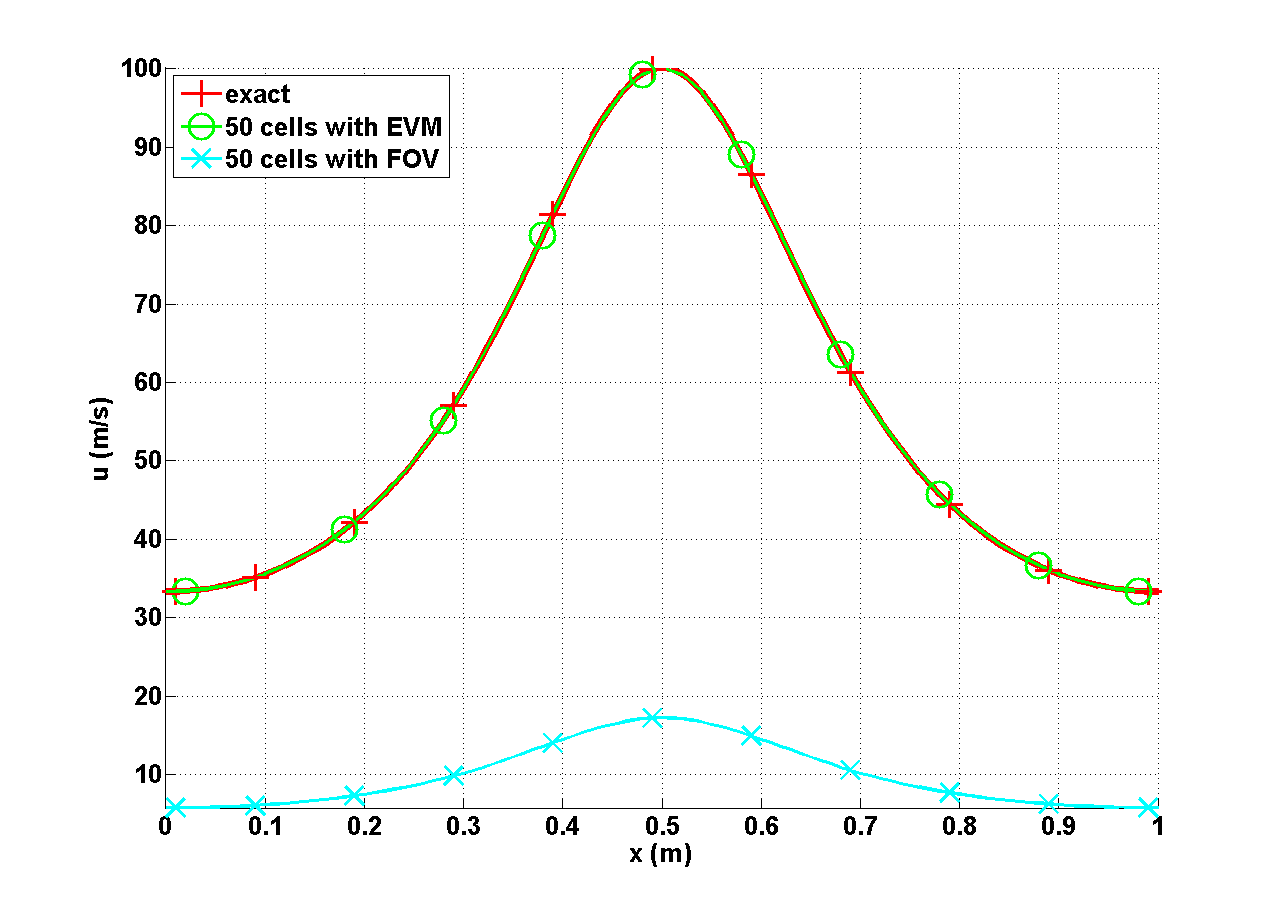
\includegraphics[width=\textwidth]{liquid_velocity_numerical_and_exact_50.png}
                \caption{Velocity solution at steady-state.}
                \label{fig:1d_nozzle_liq_vel}
        \end{subfigure}%
        %add desired spacing between images, e. g. ~, \quad, \qquad etc. 
          %(or a blank line to force the subfigure onto a new line)
        \begin{subfigure}[b]{0.495\textwidth}
                \centering
                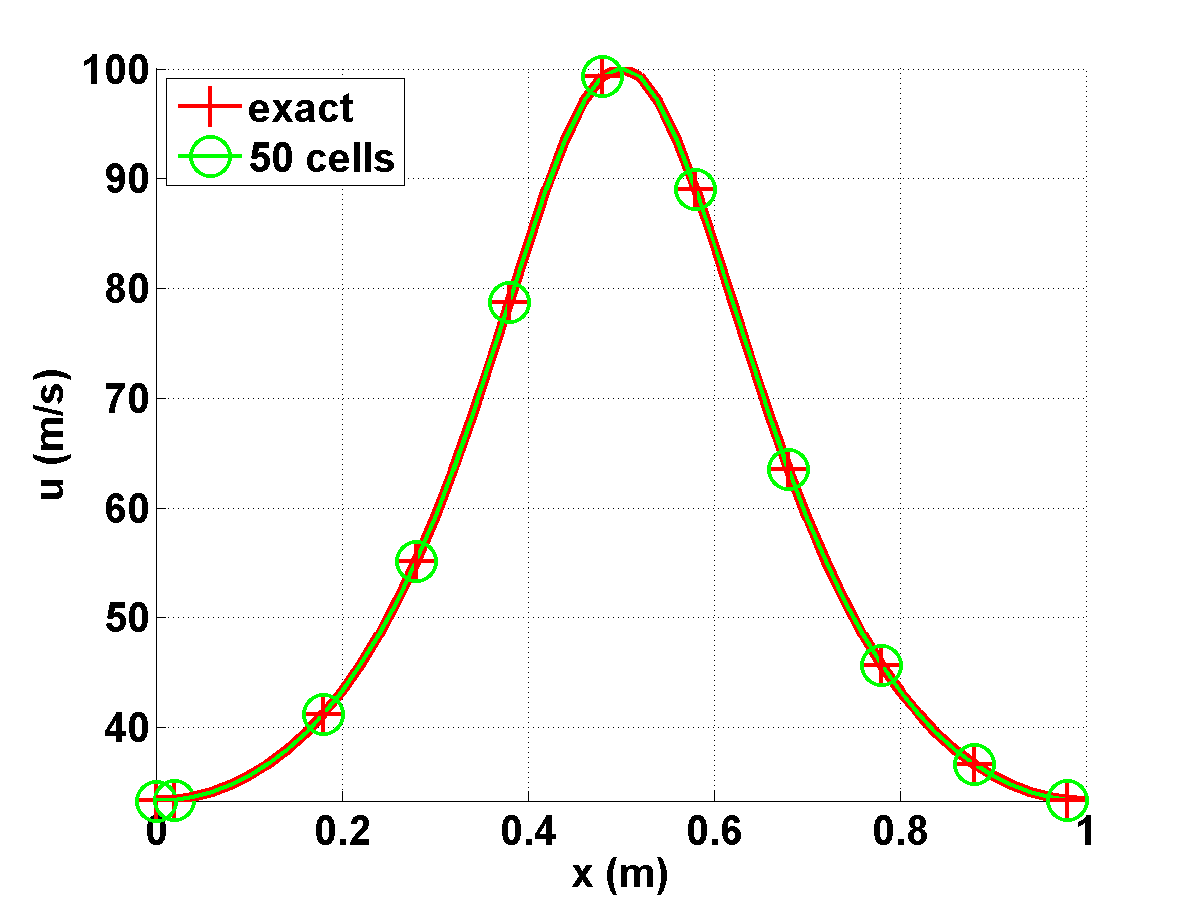
\includegraphics[width=\textwidth]{liquid_density_numerical_and_exact_50.png}
                \caption{Density solution at steady-state}
                \label{fig:1d_nozzle_liq_density}
        \end{subfigure}
        
         %add desired spacing between images, e. g. ~, \quad, \qquad etc. 
          %(or a blank line to force the subfigure onto a new line)
        \begin{subfigure}[b]{0.495\textwidth}
                \centering
                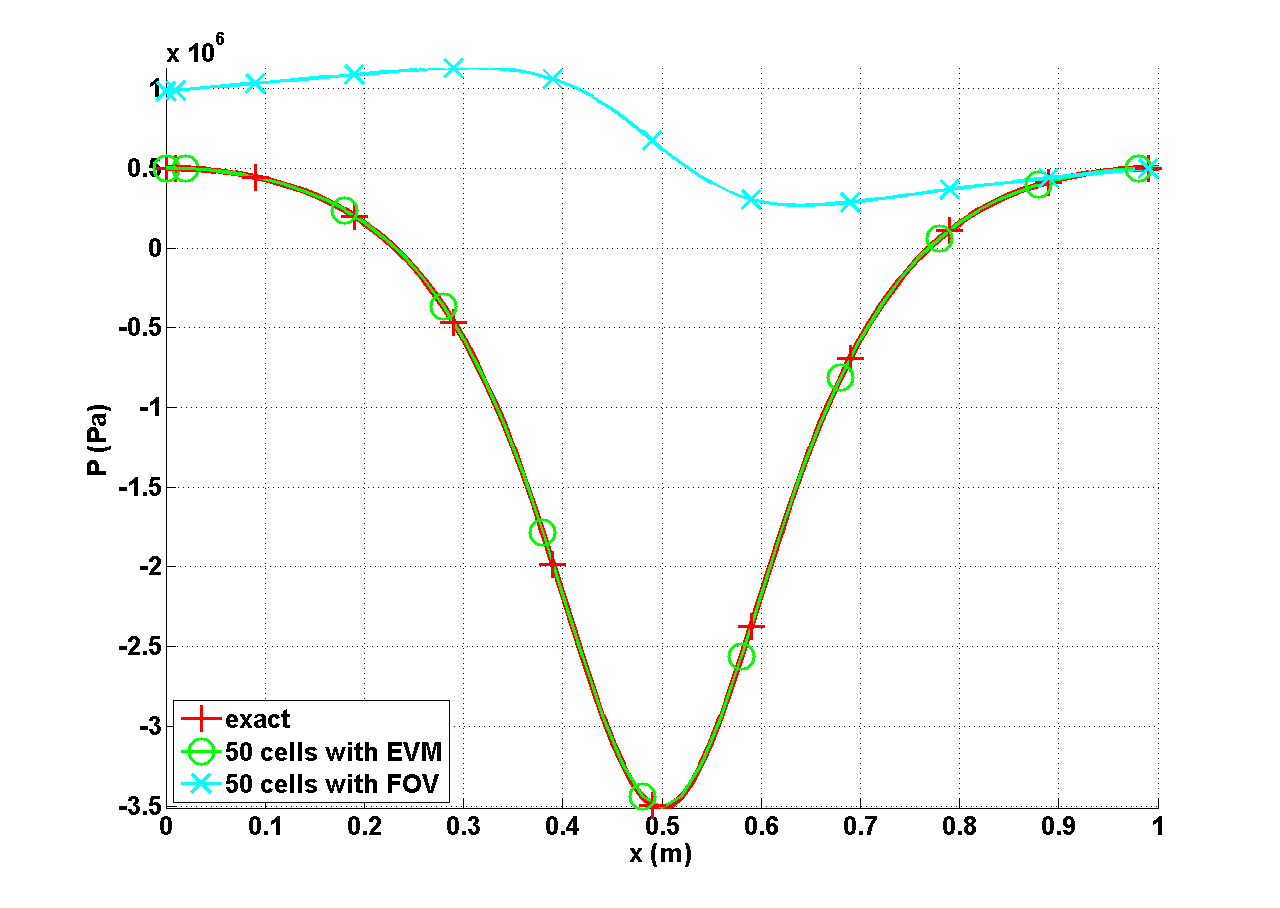
\includegraphics[width=\textwidth]{liquid_pressure_numerical_and_exact_50.png}
                \caption{Pressure solution at steady-state.}
                \label{fig:1d_nozzle_liq_press}
        \end{subfigure}
          %add desired spacing between images, e. g. ~, \quad, \qquad etc. 
          %(or a blank line to force the subfigure onto a new line)
        \begin{subfigure}[b]{0.495\textwidth}
                \centering
                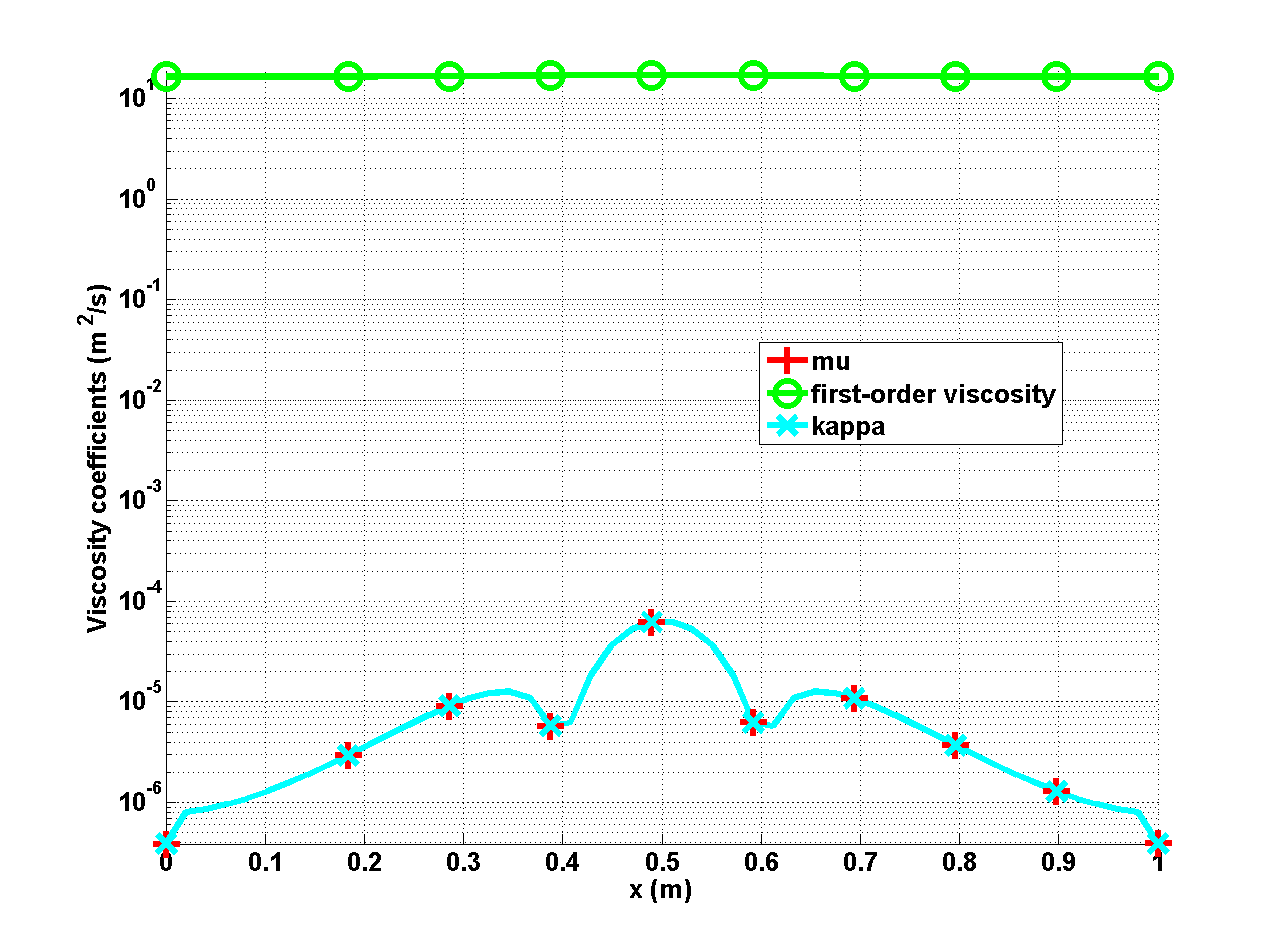
\includegraphics[width=\textwidth]{liquid_viscosity_numerical50.png}
                \caption{Viscosity coefficients at steady-state.}
                \label{fig:1d_nozzle_liq_visc}
        \end{subfigure}
        \caption{Steady-state solution for liquid phase in a $1$-D convergent-divergent nozzle with an uniform mesh of $50$ cells.}\label{fig:1d_liq_nozzle}
\end{figure}
The numerical and exact solutions of the velocity, pressure and density given in \fig{fig:1d_liq_nozzle} for a fairly coarse mesh ($50$ cells) perfectly overlap: it is noted the symmetry of the numerical solution with respect to the nozzle throat located in $x=0.5m$. The second-order viscosity coefficient  is very small compare to the first-order one as expected, since the numerical solution is smooth as shown in \fig{fig:1d_nozzle_liq_visc}. A study convergence was performed using the exact solution as a reference: the L$2$ norm of the error and the corresponding convergence rates are computed at steady-state on various uniform mesh from $4$ to $256$ cells. The results for linear polynomials $\mathbb{Q}_1$ is reported in \tbl{tbl:l2_norm_liq}.
\begin{table}[H]
\begin{center}
 \caption{\label{tbl:l2_norm_liq} L$2$ norm of the error for the liquid phase in a $1$-D convergent-divergent nozzle at steady-state.}
 \begin{tabular}{|c|c|c|c|c|c|c|c|c|}
 \hline
   cells & density & rate & pressure & rate & velocity & rate \\
 \hline
$4$ &   $3.106397$ $10^{-1}$ & $-$ & $5.254445$ $10^{5}$ & $-$ & $3.288543$                   & $-$\\
  \hline
$8$  &  $7.491623$ $10^{-2}$ & $2.07$ & $1.636966$ $10^{5}$ & $1.60$ & $1.823880$                   & $0.90$\\
   \hline
$16$ & $2.079858$ $10^{-2}$ & $1.80$ & $4.627338$ $10^{4}$ & $1.75$ & $4.990605$ $10^{-1}$ & $1.83$\\
 \hline
$32$ & $5.329627$ $10^{-3}$ & $1.90$ & $1.180287$ $10^{4}$ & $1.92$ & $1.261018$ $10^{-1}$ & $1.93$\\
 \hline
$64$ & $1.341583$ $10^{-3}$ & $1.94$ & $2.967104$ $10^{3}$ & $1.98$ & $3.160914$ $10^{-2}$ & $1.99$\\
 \hline
$128$&$3.359766$ $10^{-4}$ & $1.99$ & $7.428087$ $10^{2}$ & $1.99$ & $7.907499$ $10^{-3}$ & $1.99$\\
 \hline
$256$&$8.403859$ $10^{-5}$& $1.99$ & $1.857861$ $10^{2}$ & $1.99$ & $1.977292$ $10^{-3}$ & $1.99$\\
 \hline
\end{tabular}
\end{center}
\nonumber
\end{table}
It is observed that the convergence rate for the L$2$ norm of the error is $2$: the entropy viscosity method conserves the high-order accuracy when the numerical solution is smooth, and the new definition of the entropy viscosity coefficient seems to behave as expected in the low Mach limit.
%---------------------------------------------------------------------------------------------------
\subsection{Steam in a $1$-D divergent-convergent nozzle} \label{sec:steam_nozzle}
%---------------------------------------------------------------------------------------------------
The results of this section are obtained using the exact same $1$-D geometry, initial condition and boundary conditions as in \sct{sec:liquid_nozzle}. The Stiffened gas equation of state is still used but with different parameters that are given in \tbl{tbl:stff_gas_eos_vap}. 
\begin{table}[H]
\begin{center}
 \caption{\label{tbl:stff_gas_eos_vap} Stiffened Gas Equation of State parameters for steam.}
 \begin{tabular}{|c|c|c|c|}
 \hline
$\gamma$ & $C_v$ $(J\cdot kg^{-1} \cdot K^{-1})$ & $P_{\infty}$ $(Pa)$ & $q$ $(J \cdot kg^{-1})$ \\
 \hline
1.43 & 1040 & 0 & $2030.10^3$   \\
 \hline
\end{tabular}
\end{center}
\end{table}
The pressure difference applied between the inlet and outlet will make the steam accelerates through the nozzle and result in the formation of shock in the divergent part. The behavior is different from what is observed for the liquid water phase in \sct{sec:liquid_nozzle} because of the liquid to gas density ratio that is of $1000$. The objective of this section is to show that using the new definition of the viscosity coefficient in \eqt{eq:final_def_visc_coeff}, the shock can be correctly resolved and all spurious oscillations removed. The steady-state numerical solution is shown in \fig{fig:1d_vap_nozzle} and was run with a mesh of $1600$ cells.
\begin{figure}[H]
        \centering
        \begin{subfigure}[b]{0.495\textwidth}
                \centering
                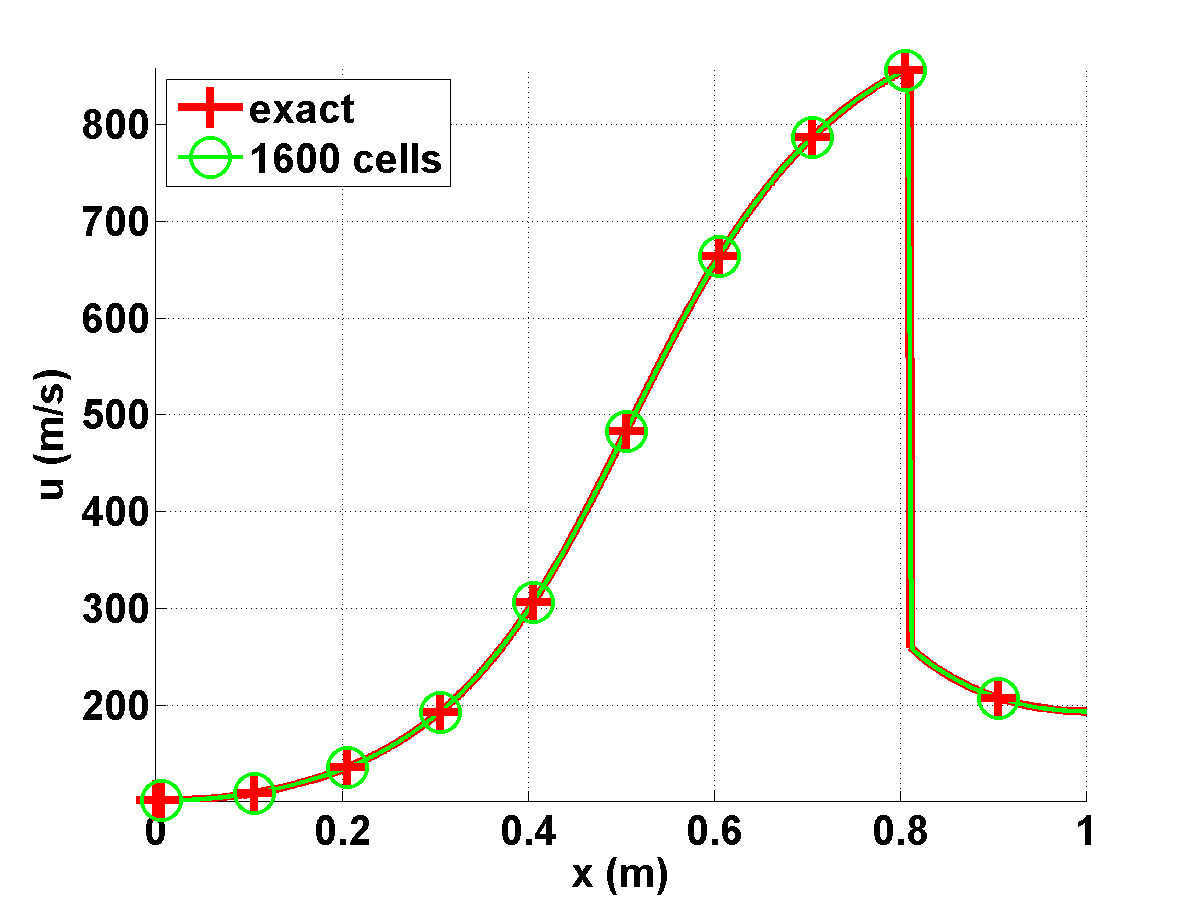
\includegraphics[width=\textwidth]{vapor_velocity_numerical_and_exact_1600.png}
                \caption{Velocity solution at steady-state.}
                \label{fig:1d_nozzle_vap_vel}
        \end{subfigure}%
        %add desired spacing between images, e. g. ~, \quad, \qquad etc. 
          %(or a blank line to force the subfigure onto a new line)
        \begin{subfigure}[b]{0.495\textwidth}
                \centering
                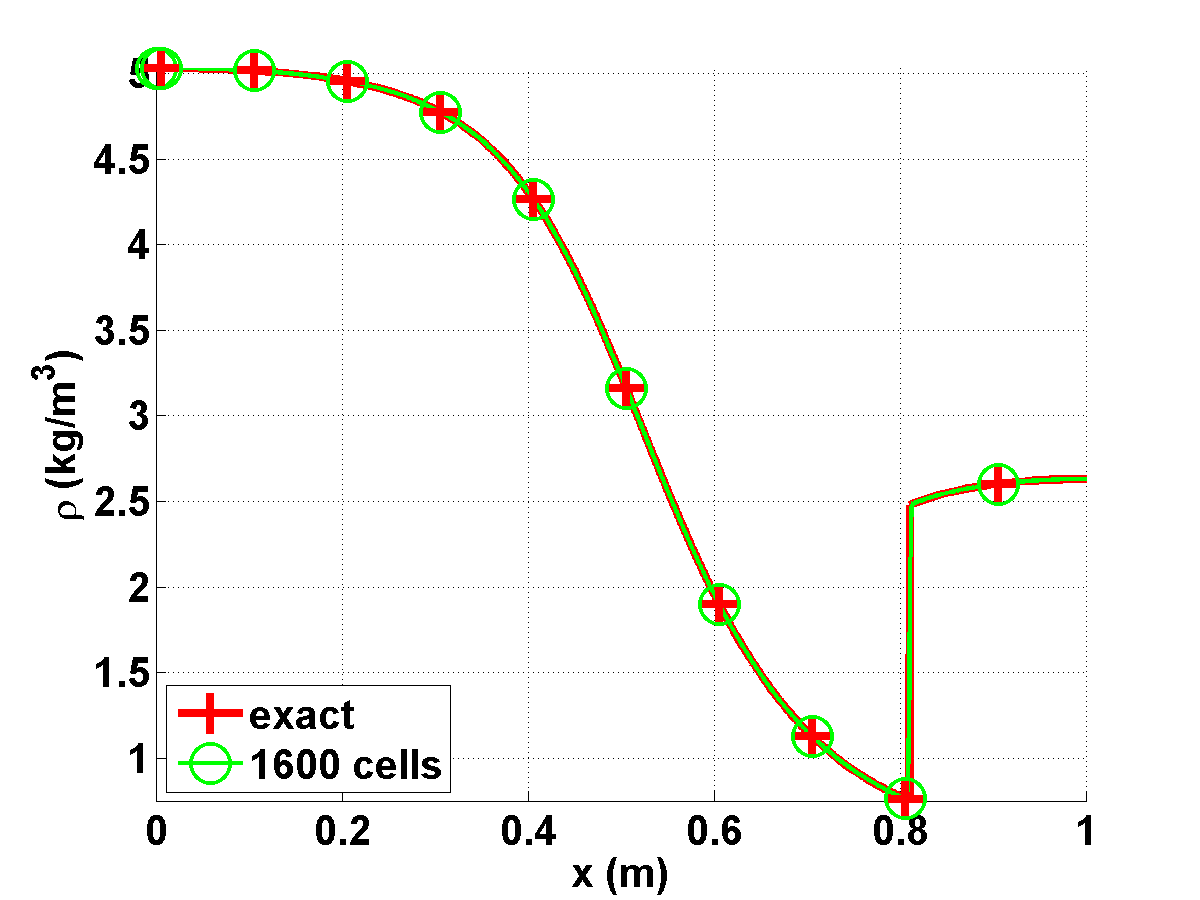
\includegraphics[width=\textwidth]{vapor_density_numerical_and_exact_1600.png}
                \caption{Density solution at steady-state}
                \label{fig:1d_nozzle_vap_density}
        \end{subfigure}
        
         %add desired spacing between images, e. g. ~, \quad, \qquad etc. 
          %(or a blank line to force the subfigure onto a new line)
        \begin{subfigure}[b]{0.495\textwidth}
                \centering
                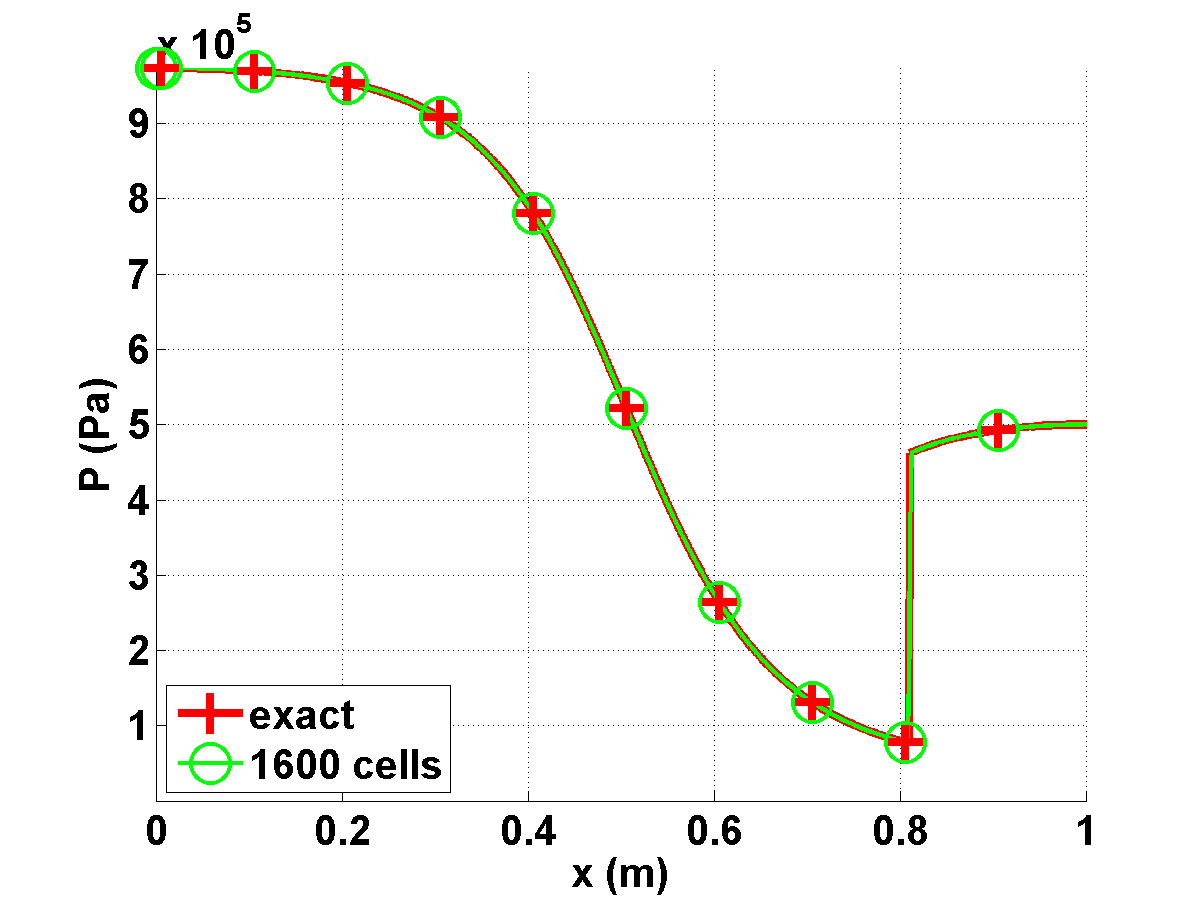
\includegraphics[width=\textwidth]{vapor_pressure_numerical_and_exact_1600.png}
                \caption{Pressure solution at steady-state.}
                \label{fig:1d_nozzle_vap_press}
        \end{subfigure}
          %add desired spacing between images, e. g. ~, \quad, \qquad etc. 
          %(or a blank line to force the subfigure onto a new line)
        \begin{subfigure}[b]{0.495\textwidth}
                \centering
                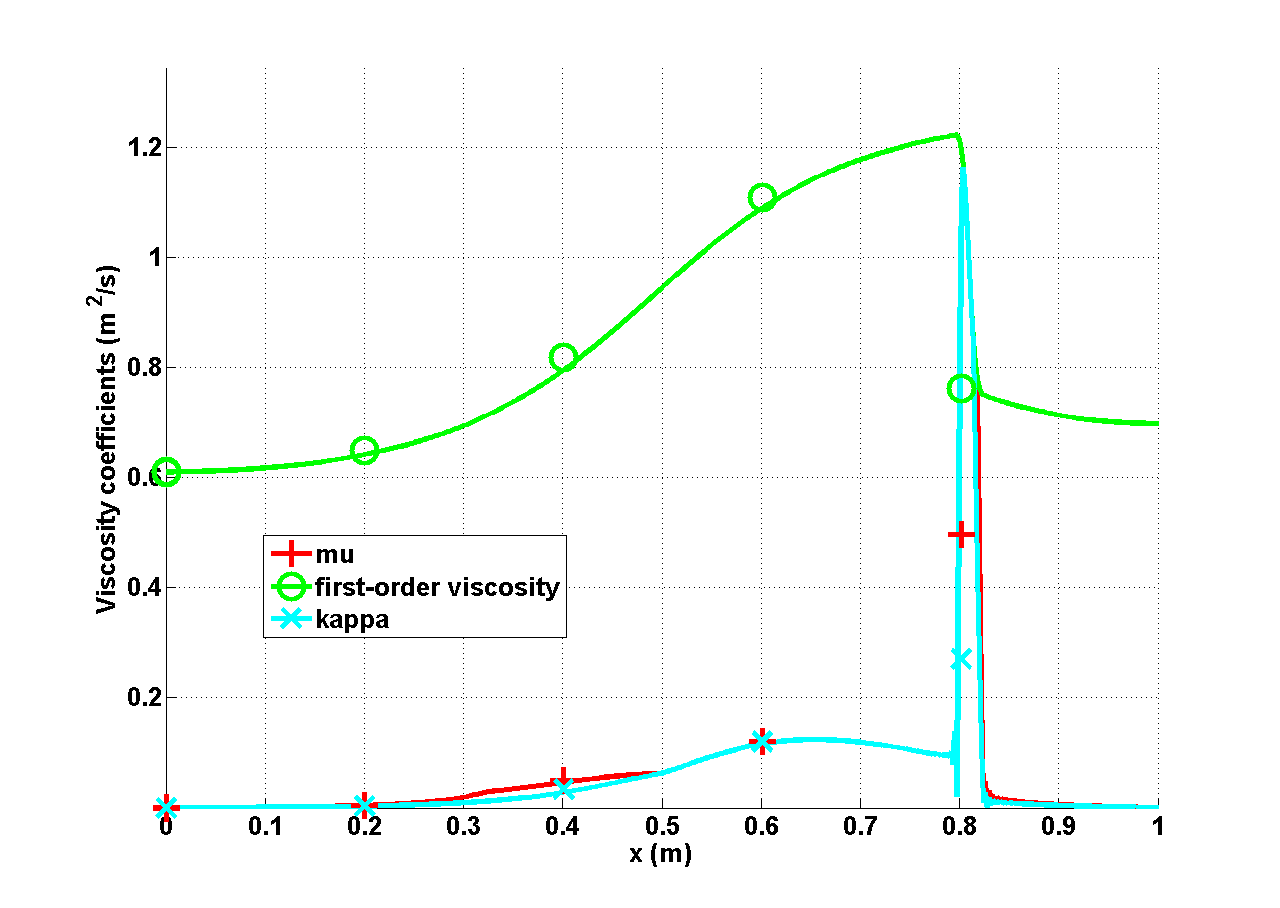
\includegraphics[width=\textwidth]{vapor_viscosity_numerical1600.png}
                \caption{Viscosity coefficients at steady-state.}
                \label{fig:1d_nozzle_vap_visc}
        \end{subfigure}
        \caption{Steady-state solution for vapor phase in a $1$-D convergent-divergent nozzle.}\label{fig:1d_vap_nozzle}
\end{figure}
The steady-state solution of the density, velocity and pressure are given in \fig{fig:1d_nozzle_vap_vel}, \fig{fig:1d_nozzle_vap_density} and \fig{fig:1d_nozzle_vap_press}. The steady-solution displays a shock around $x=0.8m$ and match the exact solution. In \fig{fig:1d_nozzle_vap_visc}, the first- and second-order viscosity coefficients are log plotted at steady-state: the second-order viscosity coefficient is peaked in the shock region around $x-0.8m$ as expected, and saturate to the first-order viscosity coefficient. The profile also displays another peak at $x=0.5m$ that corresponds to the position of the sonic point for a $1$-D convergent-divergent nozzle: this particular point is known to develop small instabilities that are detected when computing the jumps of the pressure and density gradients. Anywhere else, the second-order viscosity coefficient is small. In order to prove convergence of the numerical solution of the exact solution, a convergence study was performed. Because of the presence of a shock, second-order accuracy cannot be achieved. However, the convergence rate is known and expected to be of $1/2$ when computing the L$2$ norm of the error. Results are provided in ...
\begin{figure}[H]
\centering
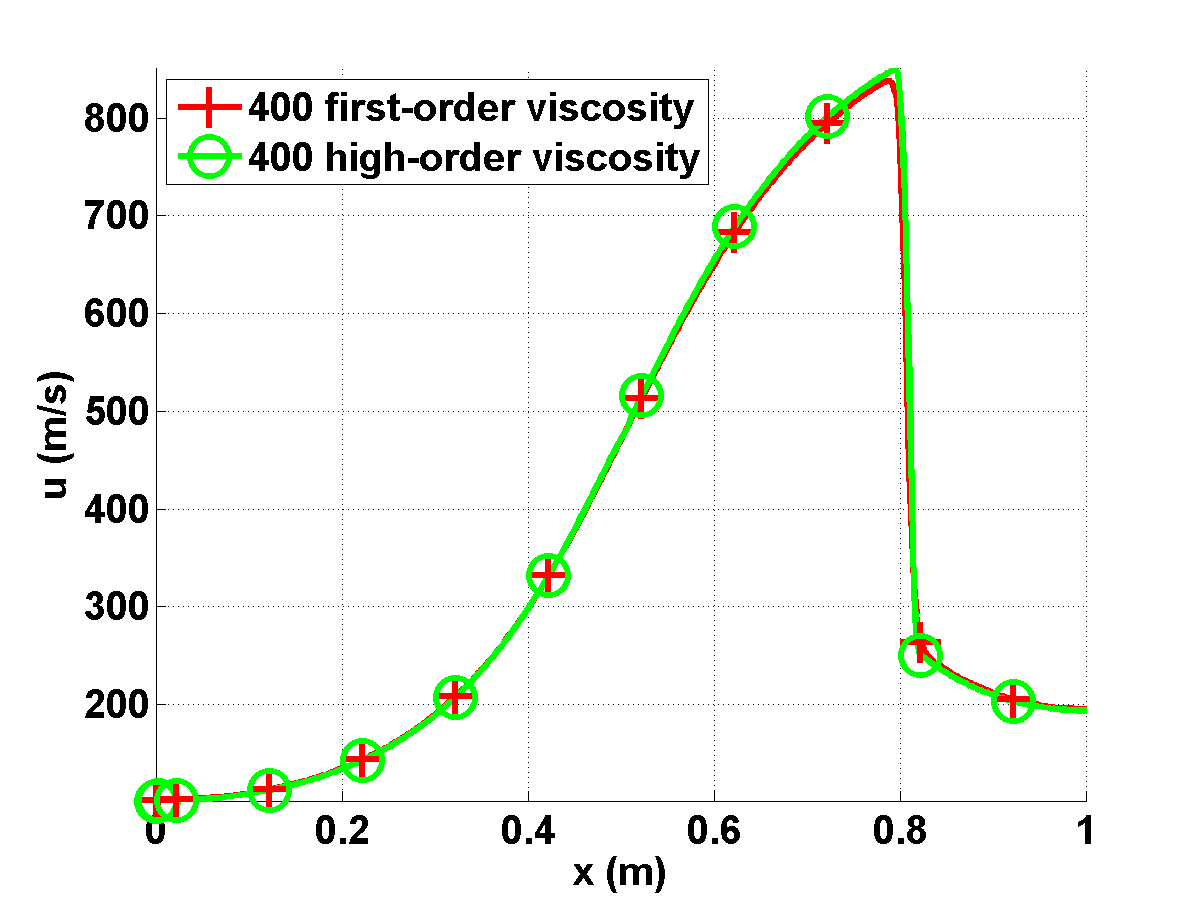
\includegraphics[width=\textwidth]{vapor_velocity_fo_and_ev_400.png}
\caption{Velocity profile at steady-state with the first- and second-order viscosity for a mesh with $400$ cells.}
\label{fig:1d_nozzle_vap_fo_ev}
\end{figure}
In \fig{fig:1d_nozzle_vap_fo_ev}, the steady-state velocity profile is plotted when using the first- and second-order viscosity coefficients: the main difference between the two numerical solution is in the resolution of the shock around $x=0.8m$. The first-order viscosity coefficient is by definition more dissipative and will smooth out the solution. In the other hand, the high-order viscosity better resolves the shock and allow high-order accuracy away from the shock region. It is also noted that the numerical solution obtained with the first-order viscosity coefficient is satisfying: this is due to the nature of the solution that contains a standing shock, and thus, will force the shock formation. 
%---------------------------------------------------------------------------------------------------
\subsection{Leblanc shock tube} \label{sec:Leblanc}
%---------------------------------------------------------------------------------------------------
\begin{table}[H]
\begin{center}
 \caption{\label{tbl:l2_norm_leblanc} L$2$ norm of the error for the $1$-D Leblanc test at $t=4.s$.}
 \begin{tabular}{|c|c|c|c|c|c|c|c|c|}
 \hline
   cells & density & rate & pressure & rate & velocity & rate \\
 \hline
$500$ &   $3.106397$ $10^{-1}$ & $-$ & $5.254445$ $10^{5}$ & $-$ & $3.288543$                   & $-$\\
  \hline
$1000$  &  $7.491623$ $10^{-2}$ & $0.64781$ & $1.636966$ $10^{5}$ & $0.58793$ & $1.823880$                   & $0.89392$\\
   \hline
$2000$ & $2.079858$ $10^{-2}$ & $0.70756$ & $4.627338$ $10^{4}$ & $0.53448$ & $0.53448$ $10^{-1}$ & $0.77533$\\
 \hline
$3000$ & $5.329627$ $10^{-3}$ & $0.64117$ & $1.180287$ $10^{4}$ & $0.58506$ & $0.58506$ $10^{-1}$ & $0.72276$\\
 \hline
$4000$ & $1.341583$ $10^{-3}$ & $0.58965$ & $2.967104$ $10^{3}$ & $0.56103$ & $0.56103$ $10^{-2}$ & $0.60112$\\
 \hline
$5000$&$3.359766$ $10^{-4}$ & $0.54925$ & $7.428087$ $10^{2}$ & $0.55095$ & $0.55095$ $10^{-3}$ & $0.55351$\\
 \hline
$6000$&$8.403859$ $10^{-5}$& $0.31882$ & $1.857861$ $10^{2}$ & $0.44813$ & $0.44813$ $10^{-3}$ & $0.15305$\\
 \hline
 $7000$&$8.403859$ $10^{-5}$& $0.51148$ & $1.857861$ $10^{2}$ & $0.52587$ & $0.52587$ $10^{-3}$ & $0.50216$\\
 \hline
 $8000$&$8.403859$ $10^{-5}$& $0.50469$ & $1.857861$ $10^{2}$ & $0.52459$ & $0.52459$ $10^{-3}$ & $0.50189$\\
 \hline
 $9000$&$8.403859$ $10^{-5}$& $0.51019$ & $1.857861$ $10^{2}$ & $0.51622$ & $0.51622$ $10^{-3}$ & $0.52773$\\
 \hline
\end{tabular}
\end{center}
\nonumber
\end{table}
\begin{figure}[H]
        \centering
        \begin{subfigure}[b]{0.495\textwidth}
                \centering
                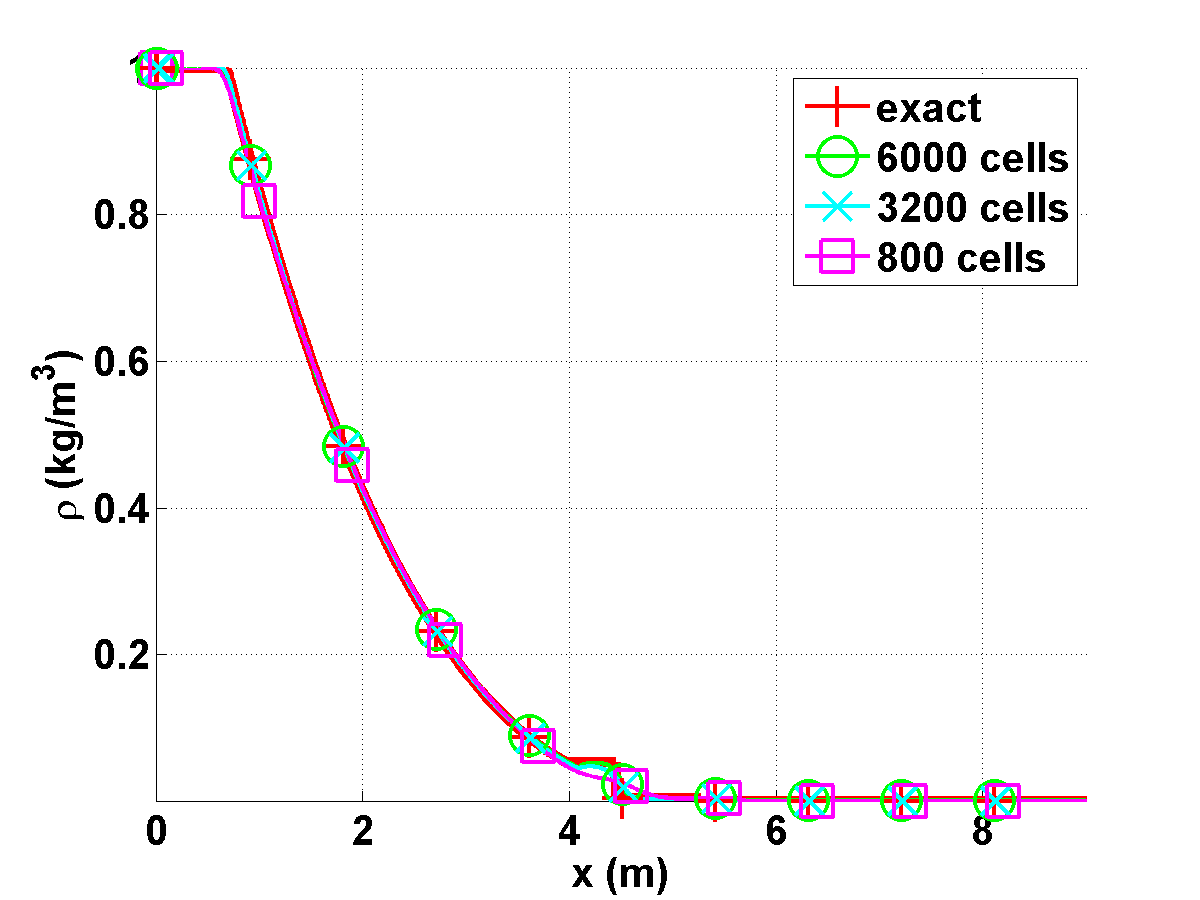
\includegraphics[width=\textwidth]{Leblanc_exact_and_numerical_stt_density_6000.png}
                \caption{Density solution at $t=4.0s$.}
                \label{fig:1d_leblanc_vel}
        \end{subfigure}%
        %add desired spacing between images, e. g. ~, \quad, \qquad etc. 
          %(or a blank line to force the subfigure onto a new line)
        \begin{subfigure}[b]{0.495\textwidth}
                \centering
                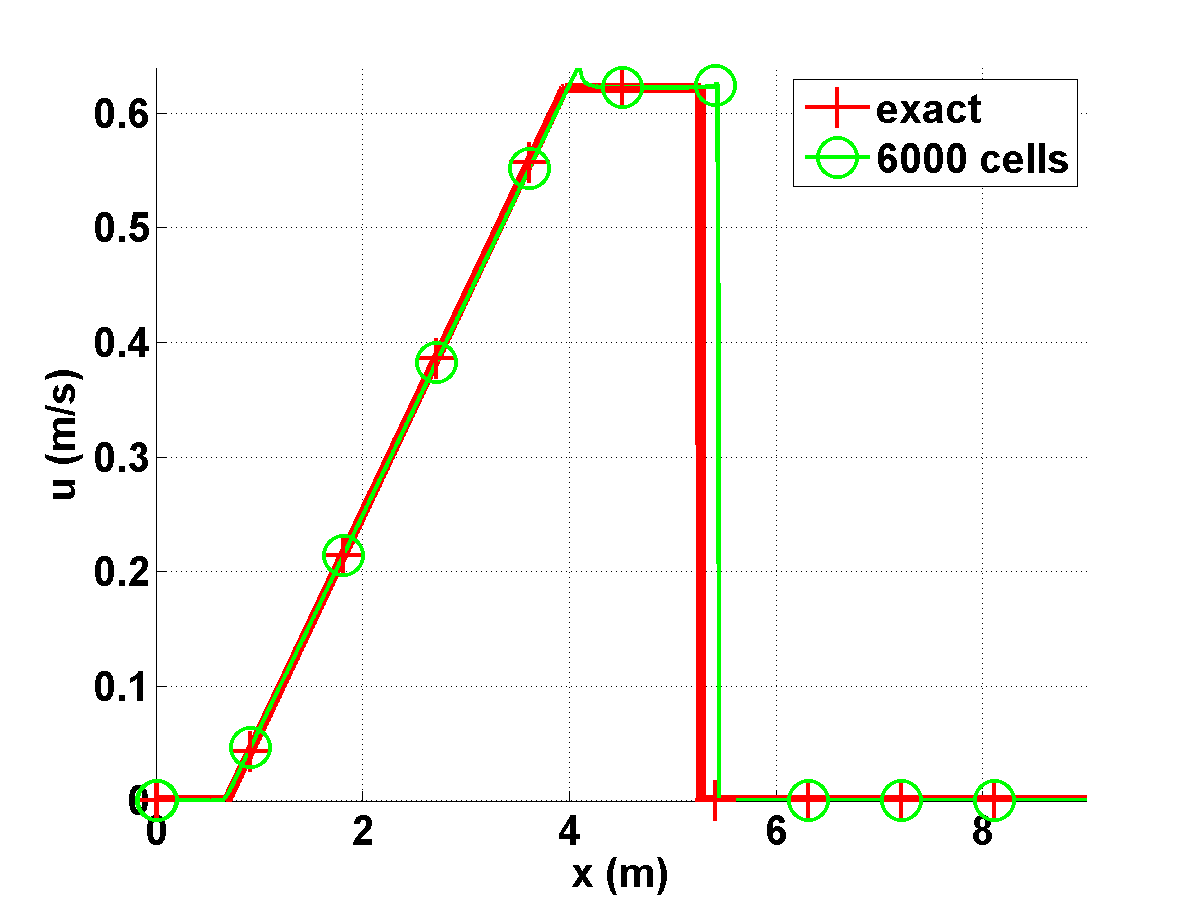
\includegraphics[width=\textwidth]{Leblanc_exact_and_numerical_stt_velocity_6000.png}
                \caption{Velocity solution at $t=4.0s$}
                \label{fig:1d_leblanc_density}
        \end{subfigure}
        
         %add desired spacing between images, e. g. ~, \quad, \qquad etc. 
          %(or a blank line to force the subfigure onto a new line)
        \begin{subfigure}[b]{0.495\textwidth}
                \centering
                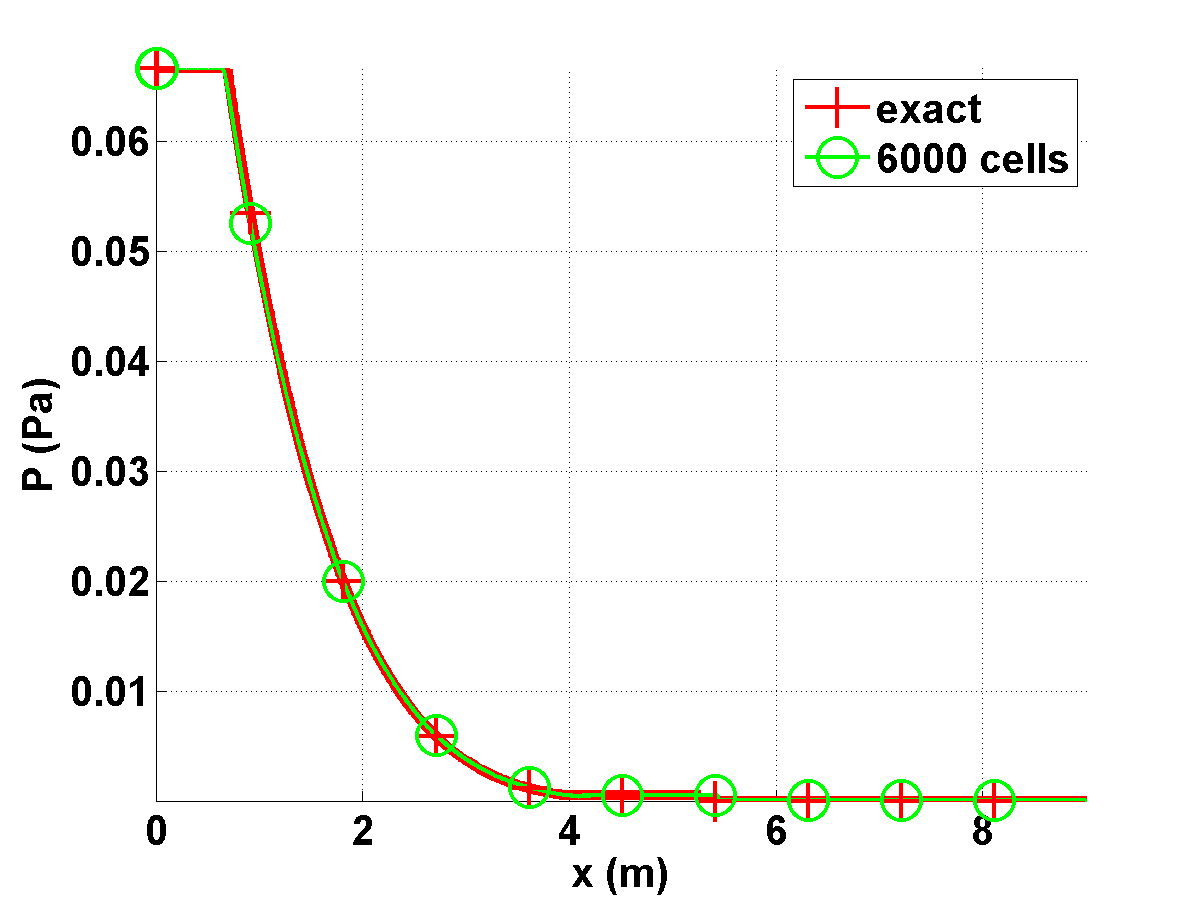
\includegraphics[width=\textwidth]{Leblanc_exact_and_numerical_stt_pressure_6000.png}
                \caption{Pressure solution at $t=4.0s$.}
                \label{fig:1d_leblanc_press}
        \end{subfigure}
          %add desired spacing between images, e. g. ~, \quad, \qquad etc. 
          %(or a blank line to force the subfigure onto a new line)
        \begin{subfigure}[b]{0.495\textwidth}
                \centering
                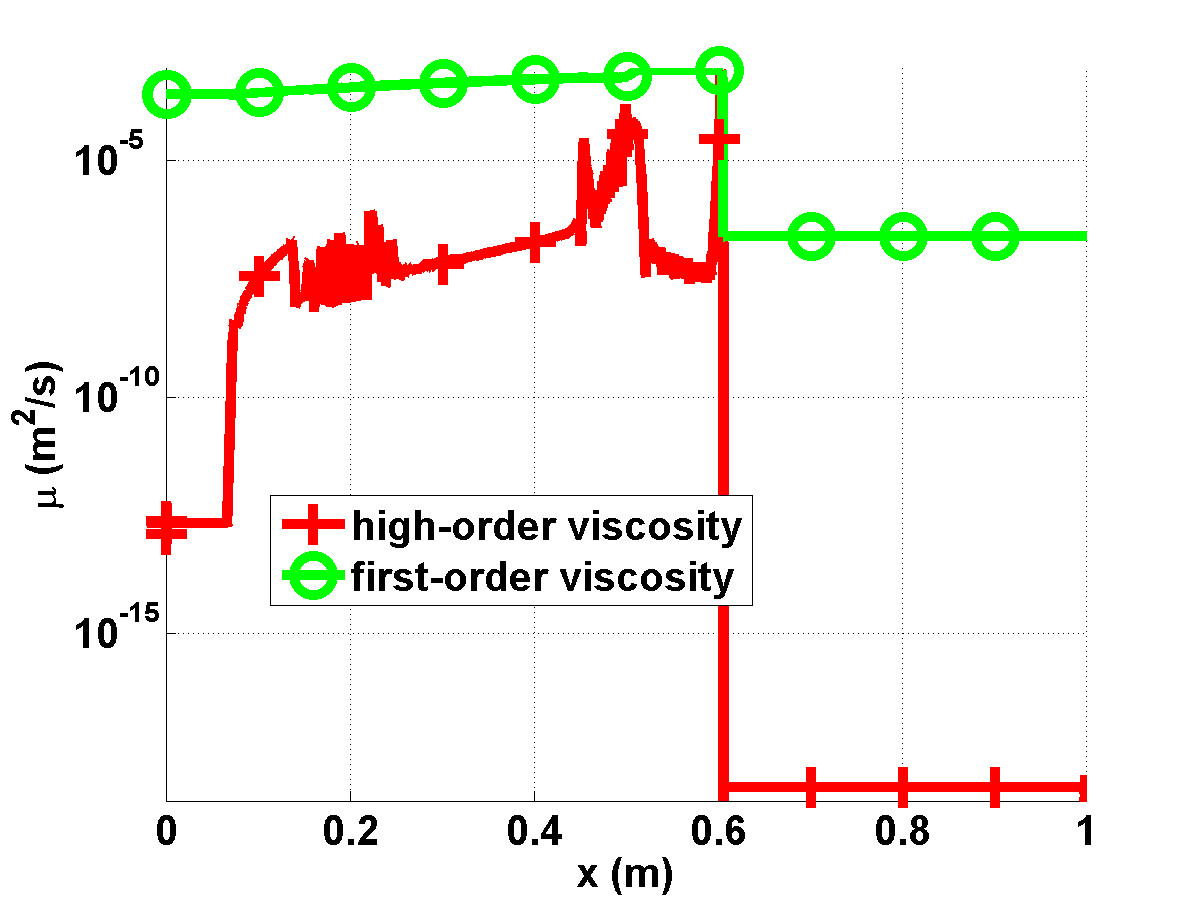
\includegraphics[width=\textwidth]{Leblanc_viscosity_numerical_6000.png}
                \caption{Viscosity coefficients at $t=4.0s$.}
                \label{fig:1d_leblanc_visc}
        \end{subfigure}
        \caption{Steady-state solution for vapor phase in a $1$-D convergent-divergent nozzle.}\label{fig:1d_lebalnc}
\end{figure}
%---------------------------------------------------------------------------------------------------
\subsection{Subsonic flow over a $2$-D cylinder} \label{sec:cylinder}
%---------------------------------------------------------------------------------------------------
\begin{figure}[H]
        \centering
        \begin{subfigure}[b]{0.495\textwidth}
                \centering
                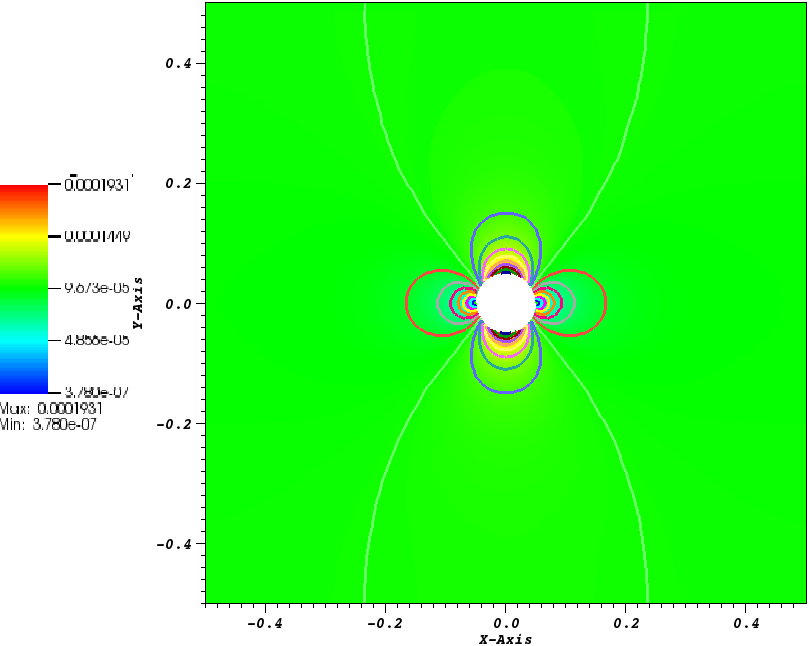
\includegraphics[width=\textwidth]{CylinderMach1em4.png}
                \caption{Velocity solution at steady-state.}
                \label{fig:cyl_1em4}
        \end{subfigure}%
        %add desired spacing between images, e. g. ~, \quad, \qquad etc. 
          %(or a blank line to force the subfigure onto a new line)
        \begin{subfigure}[b]{0.495\textwidth}
                \centering
                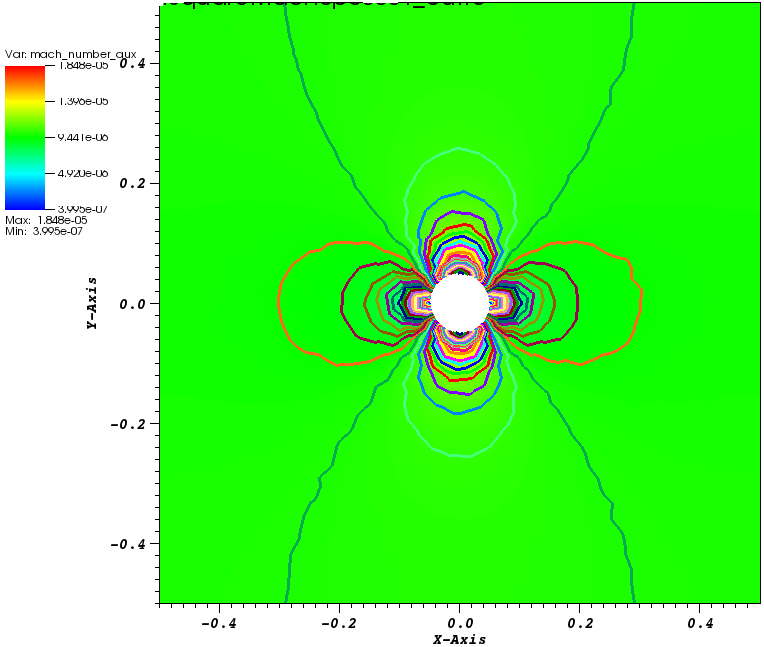
\includegraphics[width=\textwidth]{CylinderMach1em5.png}
                \caption{Density solution at steady-state}
                \label{fig:cyl_1em5}
        \end{subfigure}
        
         %add desired spacing between images, e. g. ~, \quad, \qquad etc. 
          %(or a blank line to force the subfigure onto a new line)
        \begin{subfigure}[b]{0.495\textwidth}
                \centering
                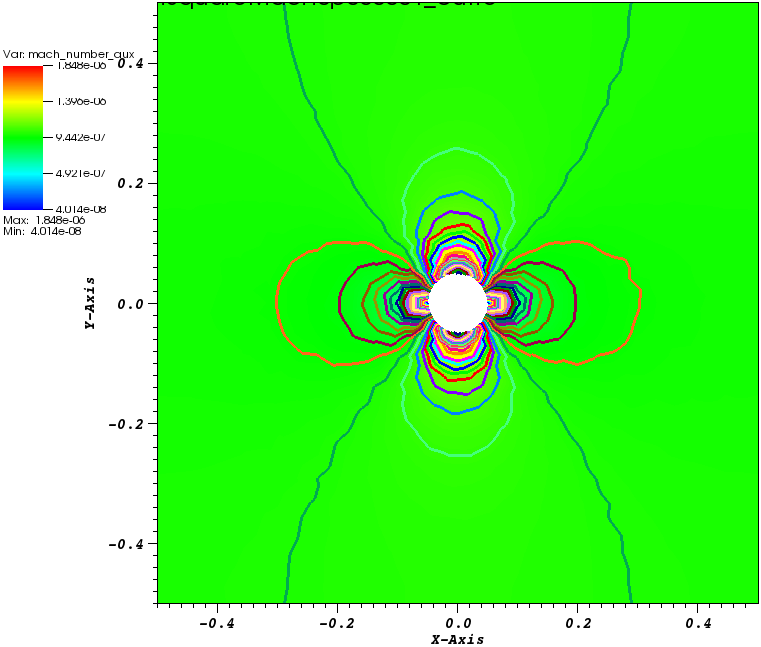
\includegraphics[width=\textwidth]{CylinderMach1em6.png}
                \caption{Presolution at steady-state.}
                \label{fig:cyl_1em6}
        \end{subfigure}
          %add desired spacing between images, e. g. ~, \quad, \qquad etc. 
          %(or a blank line to force the subfigure onto a new line)
        \begin{subfigure}[b]{0.495\textwidth}
                \centering
                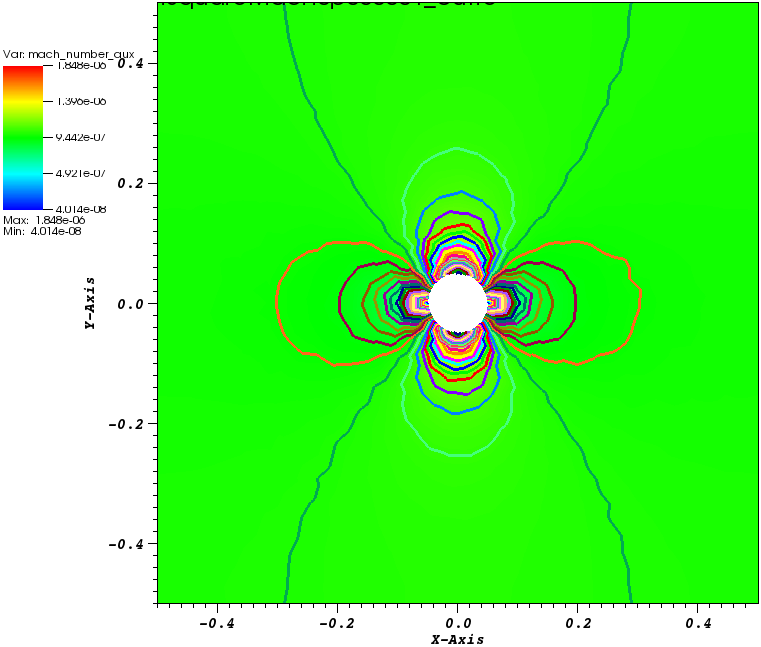
\includegraphics[width=\textwidth]{CylinderMach1em6.png}
                \caption{Viscosity coefficients.}
                \label{fig:cyl_1em7}
        \end{subfigure}
        \caption{Steady-state solution for vapor phase in a $1$-D convergent-divergent nozzle.}\label{fig:cylinder}
\end{figure}
%---------------------------------------------------------------------------------------------------
\subsection{Subsonic flow over a $2$-D hump} \label{sec:hump}
%---------------------------------------------------------------------------------------------------
\begin{figure}[H]
        \centering
        \begin{subfigure}[b]{0.5\textwidth}
                \centering
                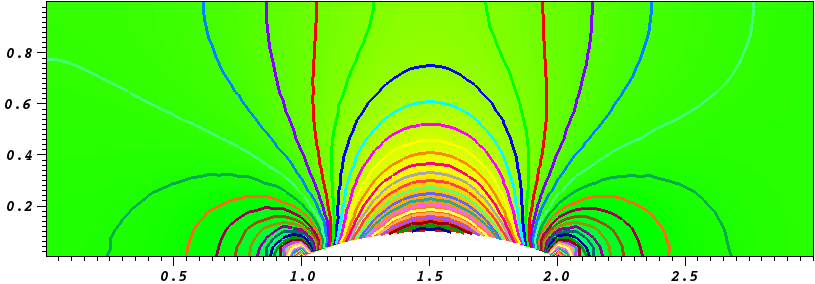
\includegraphics[width=\textwidth]{Hump2D_mach_0p01.png}
                \caption{Isomach at steady-state.}
                \label{fig:2d_hump_mach_0p01}
        \end{subfigure}%
          %add desired spacing between images, e. g. ~, \quad, \qquad etc. 
          %(or a blank line to force the subfigure onto a new line)
        \begin{subfigure}[b]{0.5\textwidth}
                \centering
                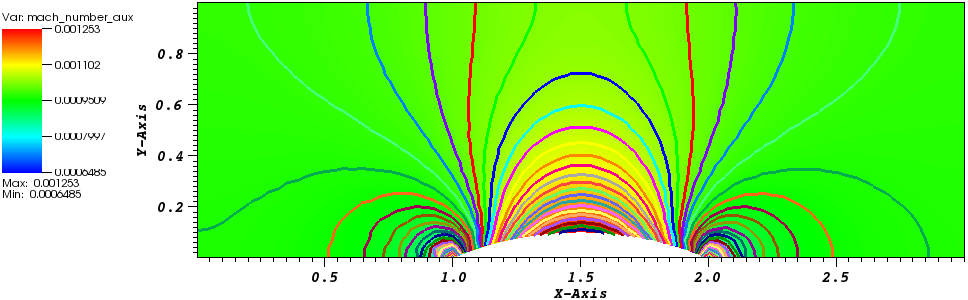
\includegraphics[width=\textwidth]{Hump2D_mach_0p001.png}
                \caption{Isomach at steady-state.}
                \label{fig:2d_hump_mach_0p001}
        \end{subfigure}%
        
        %add desired spacing between images, e. g. ~, \quad, \qquad etc. 
          %(or a blank line to force the subfigure onto a new line)
        \begin{subfigure}[b]{0.495\textwidth}
                \centering
                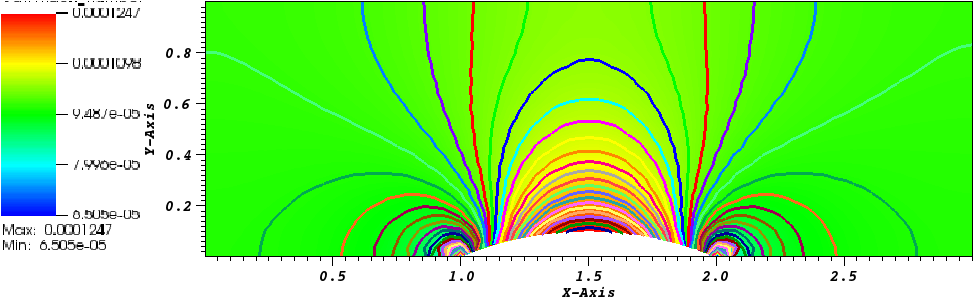
\includegraphics[width=\textwidth]{Hump2D_mach_1em4.png}
                \caption{Isomach at steady-state.}
                \label{fig:2d_hump_mach_0p0001}
        \end{subfigure}
         %add desired spacing between images, e. g. ~, \quad, \qquad etc. 
          %(or a blank line to force the subfigure onto a new line)
        \begin{subfigure}[b]{0.495\textwidth}
                \centering
                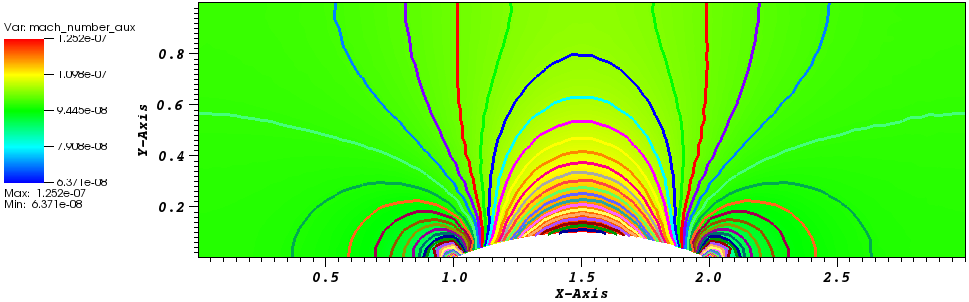
\includegraphics[width=\textwidth]{Hump2D_mach_1em7.png}
                \caption{Isomach at steady-state.}
                \label{fig:2d_hump_mach_0p0000001}
        \end{subfigure}
        \caption{Steady-state solution for a flow in a $2$-D compression corner.}\label{fig:2d_hump}
\end{figure}
%---------------------------------------------------------------------------------------------------
\subsection{Supersonic flow in a compression corner} \label{sec:corner}
%---------------------------------------------------------------------------------------------------
\begin{figure}[H]
        \centering
        \begin{subfigure}[b]{0.56\textwidth}
                \centering
                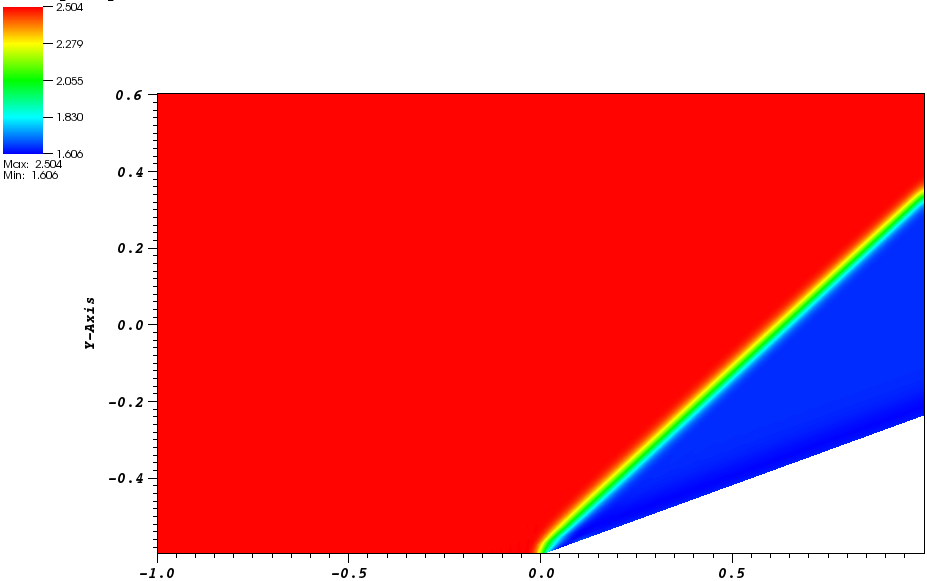
\includegraphics[width=\textwidth]{CompressionCorner2D_mach.png}
                \caption{Mach solution at steady-state.}
                \label{fig:2d_corner_mach}
        \end{subfigure}%
        %add desired spacing between images, e. g. ~, \quad, \qquad etc. 
          %(or a blank line to force the subfigure onto a new line)
        \begin{subfigure}[b]{0.5\textwidth}
                \centering
                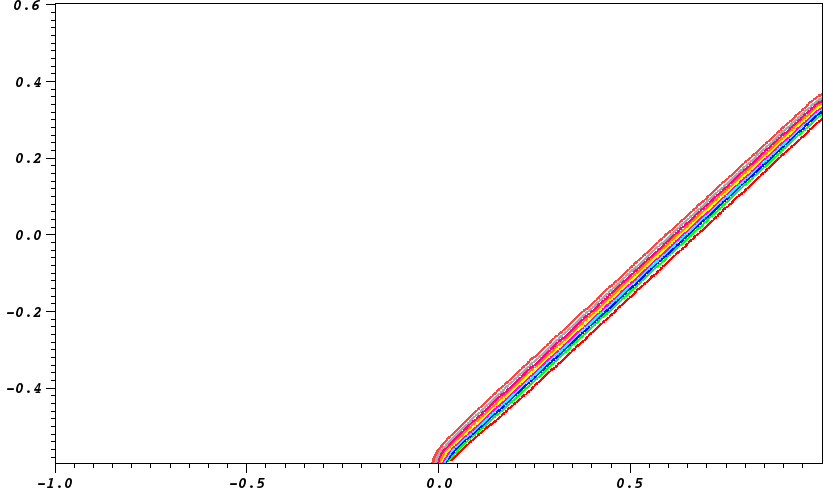
\includegraphics[width=\textwidth]{CompressionCorner2D_isomach.png}
                \caption{Isomach at steady-state}
                \label{fig:2d_corner_isomach}
        \end{subfigure}
        
         %add desired spacing between images, e. g. ~, \quad, \qquad etc. 
          %(or a blank line to force the subfigure onto a new line)
        \begin{subfigure}[b]{0.5\textwidth}
                \centering
                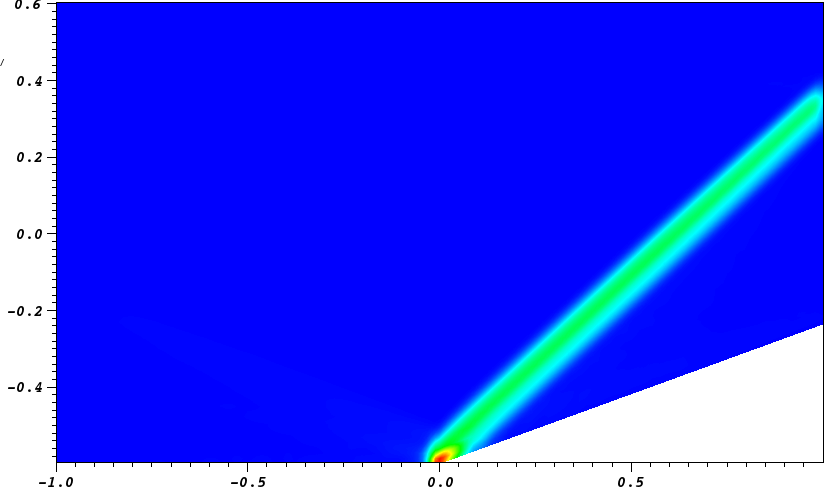
\includegraphics[width=\textwidth]{CompressionCorner2D_viscosity.png}
                \caption{Viscosity coefficient at steady-state.}
                \label{fig:2d_corner_visc}
        \end{subfigure}
        \caption{Steady-state solution for a flow in a $2$-D compression corner.}\label{fig:2d_corner}
\end{figure}
%%%%%%%%%%%%%%%%%%%%%%%%%%%%%%%%%%%%%%%%%%%%%%%%%%%%%%%%%%%%%%%%%%%%%%%%%%%%%%%%%%%%%%%%%%%%%%%%%%%%
%%%%%%%%%%%%%%%%%%%%%%%%%%%%%%%%%%%%%%%%%%%%%%%%%%%%%%%%%%%%%%%%%%%%%%%%%%%%%%%%%%%%%%%%%%%%%%%%%%%%
\section{Conclusions} \label{sec:ccl}
%%%%%%%%%%%%%%%%%%%%%%%%%%%%%%%%%%%%%%%%%%%%%%%%%%%%%%%%%%%%%%%%%%%%%%%%%%%%%%%%%%%%%%%%%%%%%%%%%%%%
%%%%%%%%%%%%%%%%%%%%%%%%%%%%%%%%%%%%%%%%%%%%%%%%%%%%%%%%%%%%%%%%%%%%%%%%%%%%%%%%%%%%%%%%%%%%%%%%%%%%


%%%%%%%%%%%%%%%%%%%%%%%%%%%%%%%%%%%%%%%%%%%%%%%%%%%%%%%%%%%%%%%%%%%%%%%%%%%%%%%%%%%%%%%%%%%%%%%%%%%%
%%%%%%%%%%%%%%%%%%%%%%%%%%%%%%%%%%%%%%%%%%%%%%%%%%%%%%%%%%%%%%%%%%%%%%%%%%%%%%%%%%%%%%%%%%%%%%%%%%%%
\section*{Acknowledgments} 
%%%%%%%%%%%%%%%%%%%%%%%%%%%%%%%%%%%%%%%%%%%%%%%%%%%%%%%%%%%%%%%%%%%%%%%%%%%%%%%%%%%%%%%%%%%%%%%%%%%%
%%%%%%%%%%%%%%%%%%%%%%%%%%%%%%%%%%%%%%%%%%%%%%%%%%%%%%%%%%%%%%%%%%%%%%%%%%%%%%%%%%%%%%%%%%%%%%%%%%%%


%%%%%%%%%%%%%%%%%%%%%%%%%%%%%%%%%%%%%%%%%%%%%%%%%%%%%%%%%%%%%%%%%%%%%%%%%%%%%%%%%%%%%%%%%%%%%%%%%%%%
%%%%%%%%%%%%%%%%%%%%%%%%%%%%%%%%%%%%%%%%%%%%%%%%%%%%%%%%%%%%%%%%%%%%%%%%%%%%%%%%%%%%%%%%%%%%%%%%%%%%
%%%%%%%%%%%%%%%%%%%%%%%%%%%%%%%%%%%%%%%%%%%%%%%%%%%%%%%%%%%%%%%%%%%%%%%%%%%%%%%%%%%%%%%%%%%%%%%%%%%%
%%%%%%%%%%%%%%%%%%%%%%%%%%%%%%%%%%%%%%%%%%%%%%%%%%%%%%%%%%%%%%%%%%%%%%%%%%%%%%%%%%%%%%%%%%%%%%%%%%%%
\pagebreak

\bibliographystyle{unsrt}
\bibliography{low_mach}
\begin{thebibliography}{11}
  \bibitem{valentin}
  \emph{Implementation of the entropy viscosity method with the discontinuous Galerkin method},
  Valentin Zingan, Jean-Luc Guermond, Jim Morel, Bojan Popov, Volume 253, 1 January 2013, Pages 479-490
 
    \bibitem{jlg}
  \emph{Viscous regularization of the Euler equations and entropy principles},
  Jean-Luc Guermond and Bojan Popov, under review.
  
    \bibitem{jlg1}
  {\em Entropy viscosity method for nonlinear conservation laws}, 
  Jean-Luc Guermond, R. Pasquetti, B. Popov, J. Comput. Phys., 230 (2011) 4248-4267.
  
    \bibitem{jlg2}
  {\em Entropy Viscosity Method for High-Order Approximations of Conservation Laws}, 
  J-L. Guermond, R. Pasquetti, 
  Lecture Notes in Computational Science and Engineering, Springer, Volume 76, (2011) 411-418.
  
   \bibitem{jlg3}
 \emph{Entropy-based nonlinear viscosity for Fourrier approximations of conservation laws}, 
 J.-L. Guermond, R. Pasquetti, C.R. Math. Acad. Sci. Paris 346 (2008) 801�806.
  
   \bibitem{SEM}
  \emph{The discrete equation method (DEM) for fully compressible, two-phase flows in ducts of spatially varying cross-section.}
  R.Berry, R.Saurel, O. LeMetayer,
  Nuclear Engineering and Design 240 (2010) 3797-3818.
  
  \bibitem{Toro}
  \emph{Riemann Solvers and numerical methods for fluid dynamics.}
  E.F. Toro, $2^{nd}$ Edition, Springer.  
  
      \bibitem{Parabolic}
  \emph{On positivity preserving finite volume schemes for Euler equations},
  Perthane B. and Shu C-W., Numer. Math., 73(1):119-130, 1996.
\end{thebibliography}
%%%%%%%%%%%%%%%%%%%%%%%%%%%%%%%%%%%%%%%%%%%%%%%%%%%%%%%%%%%%%%%%%%%%%%%%%%%%%%%%%%%%%%%%%%%%%%%%%%%%
%%%%%%%%%%%%%%%%%%%%%%%%%%%%%%%%%%%%%%%%%%%%%%%%%%%%%%%%%%%%%%%%%%%%%%%%%%%%%%%%%%%%%%%%%%%%%%%%%%%%
\end{document}
%%%%%%%%%%%%%%%%%%%%%%%%%%%%%%%%%%%%%%%%%%%%%%%%%%%%%%%%%%%%%%%%%%%%%%%%%%%%%%%%%%%%%%%%%%%%%%%%%%%%
%%%%%%%%%%%%%%%%%%%%%%%%%%%%%%%%%%%%%%%%%%%%%%%%%%%%%%%%%%%%%%%%%%%%%%%%%%%%%%%%%%%%%%%%%%%%%%%%%%%%
